\documentclass[10pt]{article}
\usepackage[french]{babel}
\usepackage[utf8]{inputenc}
\usepackage[T1]{fontenc}
\usepackage{graphicx}
\usepackage[export]{adjustbox}
\graphicspath{ {./images/} }
\usepackage{caption}
\usepackage{amsmath}
\usepackage{amsfonts}
\usepackage{amssymb}
\usepackage[version=4]{mhchem}
\usepackage{stmaryrd}
\usepackage{array}
\usepackage{ragged2e}
\usepackage{enumitem}

\newcolumntype{L}[1]{>{\RaggedRight\arraybackslash}p{#1}}
\newcolumntype{C}[1]{>{\Centering\arraybackslash}p{#1}}
\newcolumntype{R}[1]{>{\RaggedLeft\arraybackslash}p{#1}}

\begin{document}
\captionsetup{singlelinecheck=false}
\section*{ÉPREUVE MUTUALISÉE AVEC E3A-POLYTECH \\
 ÉPREUVE SPÉCIFIQUE - FILIÈRE MP}
\section*{SCIENCES INDUSTRIELLES}
Durée : 4 heures\\
N.B. : le candidat attachera la plus grande importance à la clarté, à la précision et à la concision de la rédaction. Si un candidat est amené à repérer ce qui peut lui sembler être une erreur d'énoncé, il le signalera sur sa copie et devra poursuivre sa composition en expliquant les raisons des initiatives qu'il a été amené à prendre.

RAPPEL DES CONSIGNES

\begin{itemize}
  \item[-] Utiliser uniquement un stylo noir ou bleu foncé non effaçable pour la rédaction de votre composition ; d'autres couleurs, excepté le vert, peuvent être utilisées, mais exclusivement pour les schémas et la mise en évidence des résultats.
  \item[-] Ne pas utiliser de correcteur.
  \item[-] Écrire le mot FIN à la fin de votre composition.
\end{itemize}

Les calculatrices sont autorisées.

Le sujet est composé de cinq parties, toutes indépendantes.

Le sujet est composé de 20 pages : page 1 à 20.\\
Le Document Réponse est composé de 4 pages : DR1 à DR4 et du document D5.

Le Document Réponse doit être rendu dans son intégralité avec la copie.

\section*{Système de télé-échographie}
\section*{Présentation}
\section*{1. Mise en situation}
L'échographie est une technique d'imagerie médicale basée sur l'exploitation de la réflexion d'une onde ultrasonore au niveau des interfaces physiologiques entre organes. Non irradiante, peu coûteuse et mobile, elle représente l'examen d'imagerie médicale le plus pratiqué au monde. En contrepartie, sa réalisation nécessite un manipulateur expert en imagerie médicale, capable d'analyser les images échographiques en temps réel afin d'orienter la sonde en conséquence. L'analyse et l'expertise sont donc réalisées pendant l'examen. De ce fait, cette technique d'imagerie est qualifiée de " manipulateur dépendant " : sa mise en œuvre est difficilement envisageable sur des sites isolés.

La robotisation de cette technique permet toutefois d'en élargir le champ d'application. Grâce à la télé-échographie robotisée (figure 1), il devient possible de réaliser une échographie sur un patient situé sur un site isolé (appelé site patient), alors même que le spécialiste en imagerie médicale se trouve sur un site distant de celui où est pratiqué l'examen (appelé site expert).

\begin{figure}[h]
\begin{center}
  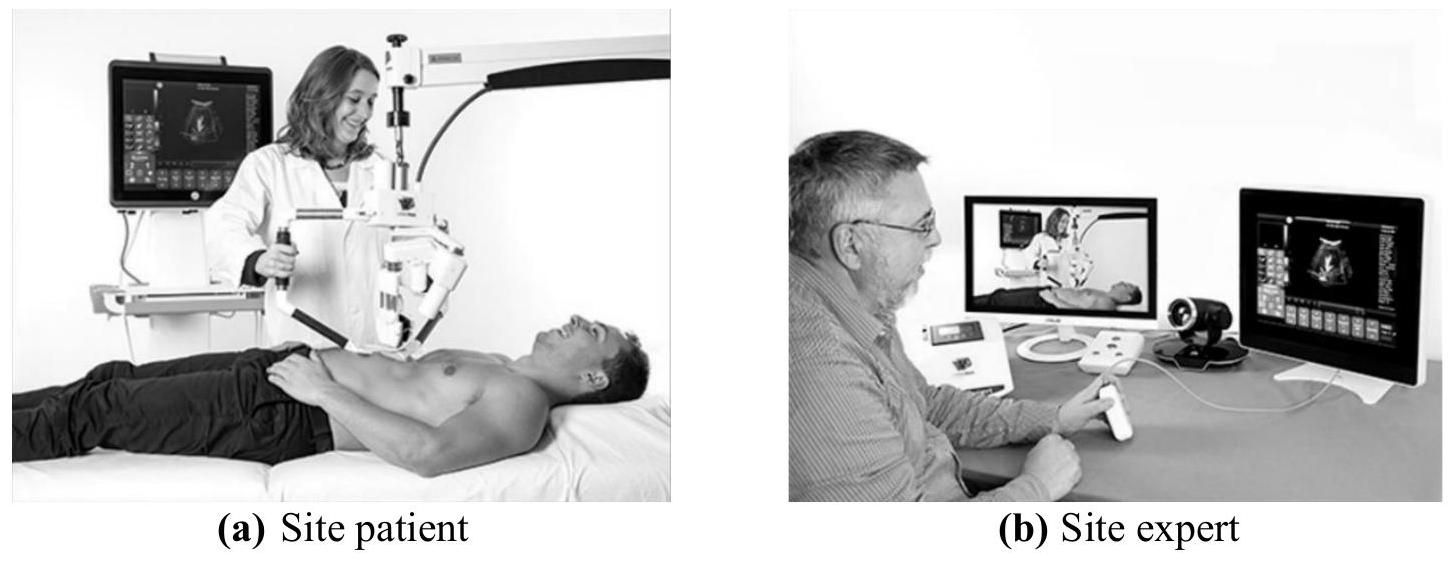
\includegraphics[alt={},max width=\textwidth]{fa0d4e8b-3d38-4fa1-81c7-d2340e1d78c1-02_561_1450_1095_343}
\captionsetup{labelformat=empty}
\caption{Figure 1 - Principe de la télé-échographie}
\end{center}
\end{figure}

Sur le site patient (figure 1a) équipé du robot porte-sonde, d'un échographe et d'un système de visioconférence, un professionnel de santé est chargé de positionner le robot porte-sonde sur le patient et de le maintenir au cours de l'examen. Depuis le site expert distant (figure 1b), le médecin dirige l'examen échographique. En manipulant une sonde fictive, il donne une consigne de position pour la sonde, que le robot exécute au contact du patient. Réalisant le lien entre les deux sites, le réseau de communication (ISDN, 4G, satellite...) permet en temps réel, le contrôle du robot, la visioconférence ainsi que la transmission des images échographiques.

\section*{2. Analyse système partielle}
Le diagramme d'exigences (D5 du document réponse), présente un extrait du cahier des charges du système de télé-échographie.

La figure 2 décrit le robot porte-sonde constitué :

\begin{itemize}
  \item[-] d'une structure porteuse 0 ;
  \item[-] d'un module de rotation, composé des sous-ensembles 1, 2, 3, permettant d'orienter la sonde en lui imposant trois rotations ( $\mathrm{R}_{1}, \mathrm{R}_{2}, \mathrm{R}_{3}$ ) suivant les axes 1 à 3 ;
  \item[-] du porte-sonde 4 sur lequel est fixé la sonde échographique S. La translation T suivant l'axe 4 permet de contrôler l'effort de contact sonde/peau du patient.
\end{itemize}

\begin{figure}[h]
\begin{center}
  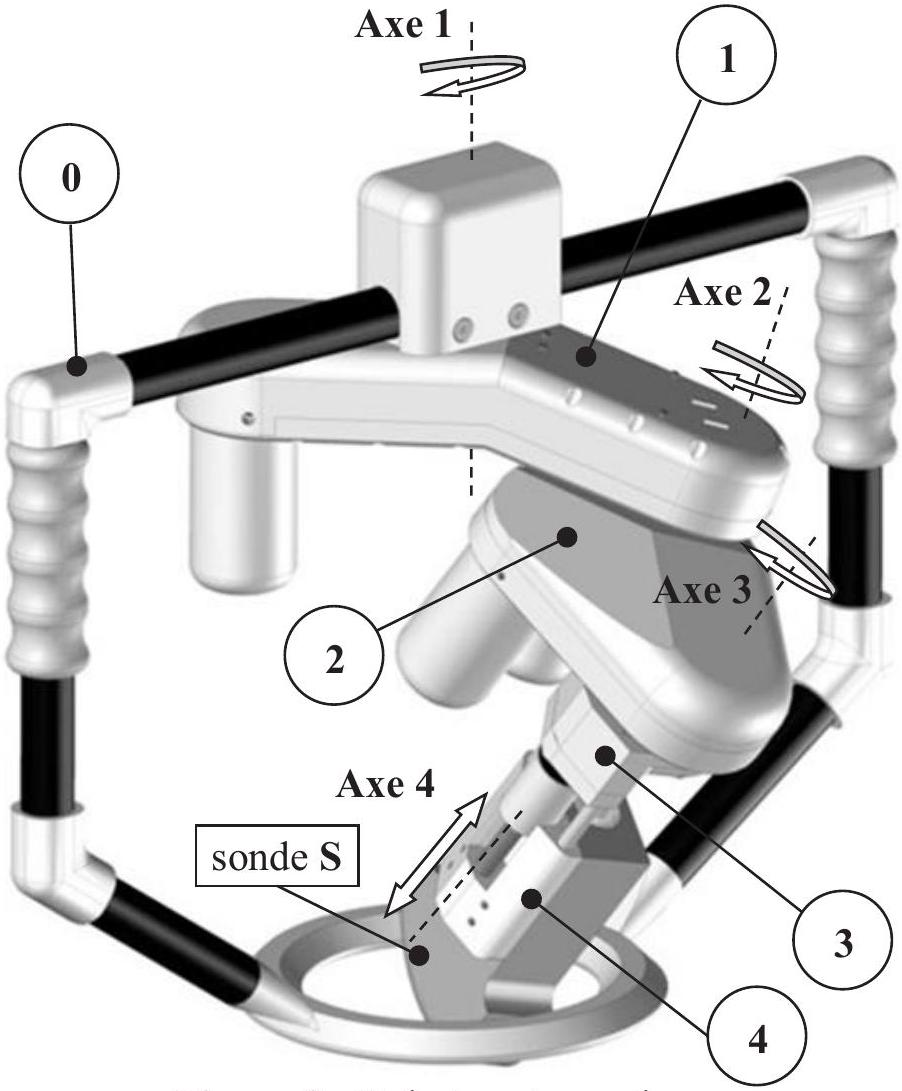
\includegraphics[alt={},max width=\textwidth]{fa0d4e8b-3d38-4fa1-81c7-d2340e1d78c1-03_1091_902_191_189}
\captionsetup{labelformat=empty}
\caption{Figure 2 - Robot porte-sonde}
\end{center}
\end{figure}

\begin{figure}[h]
\begin{center}
  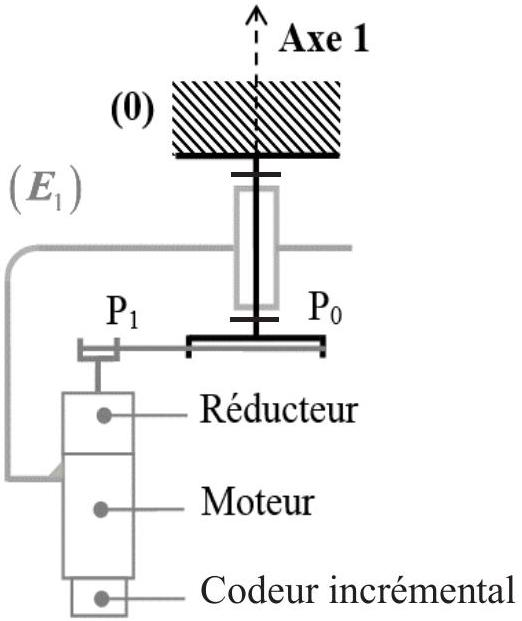
\includegraphics[alt={},max width=\textwidth]{fa0d4e8b-3d38-4fa1-81c7-d2340e1d78c1-03_621_522_189_1281}
\captionsetup{labelformat=empty}
\caption{Figure 3 - Chaîne cinématique associée à l'axe 1}
\end{center}
\end{figure}

\begin{table}[h]
\begin{center}
\begin{tabular}[t]{|l|l|}
\hline
Réducteur (R) & Rapport de réduction \( r=1 / 30,7 \) \\
\hline
Poulie $\mathrm{P}_{0}$ & Diamètre $\mathrm{D}_{0}=42 \mathrm{~mm}$ \\
\hline
Poulie $\mathrm{P}_{1}$ & Diamètre $\mathrm{D}_{1}=13 \mathrm{~mm}$ \\
\hline
\end{tabular}
\captionsetup{labelformat=empty}
\caption{Tableau 1 - Caractéristiques de la transmission}
\end{center}
\end{table}

On nomme $\boldsymbol{E}_{1}$ l'ensemble $\{\mathbf{1}, \mathbf{2}, \mathbf{3}, \mathbf{4}\}$.\\
La chaîne fonctionnelle assurant la rotation $\mathrm{R}_{1}$ de l'ensemble $\boldsymbol{E}_{1}$ autour de l'axe 1 est décrite par le schéma cinématique de la figure 3 et le diagramme de blocs internes de la figure 4.

\begin{figure}[h]
\begin{center}
  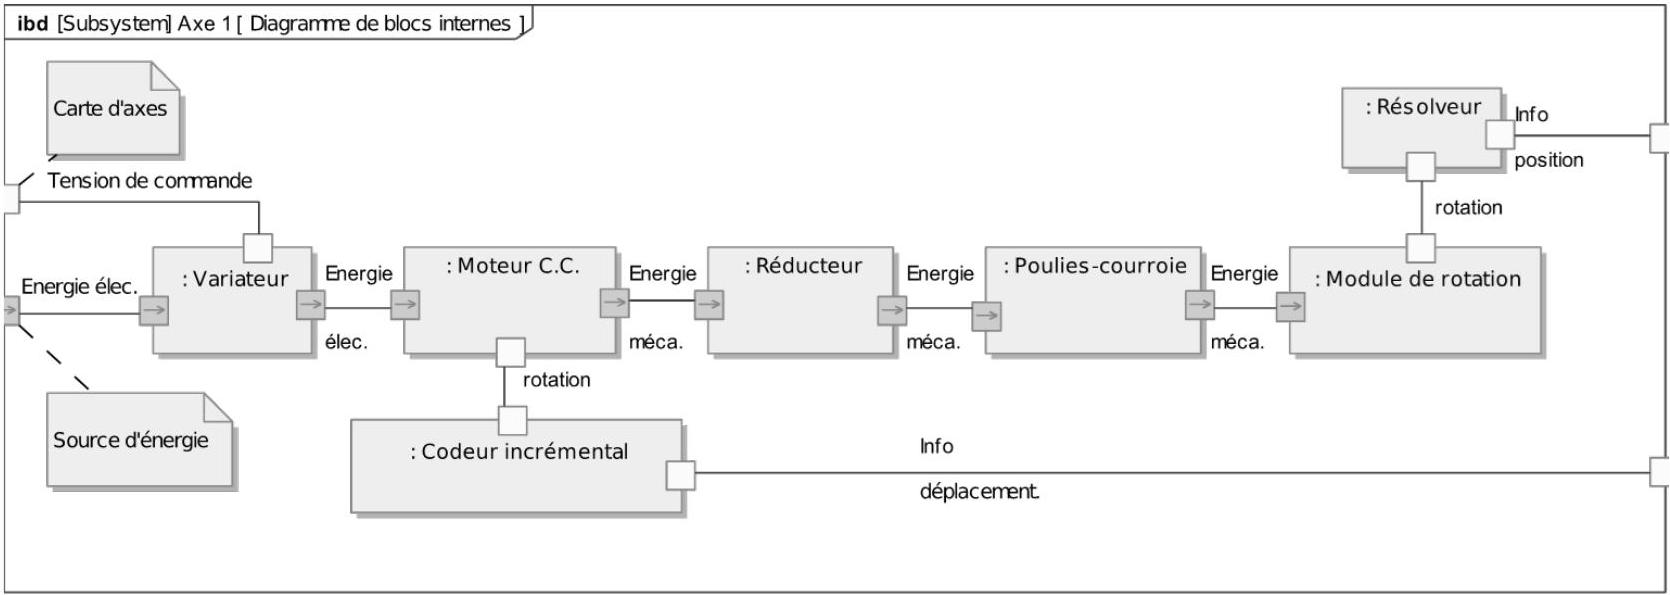
\includegraphics[alt={},max width=\textwidth]{fa0d4e8b-3d38-4fa1-81c7-d2340e1d78c1-03_595_1670_1579_193}
\captionsetup{labelformat=empty}
\caption{Figure 4 - Diagramme de blocs internes de l'axe 1}
\end{center}
\end{figure}

\section*{3. Problème posé}
Afin que le praticien soit en mesure d'obtenir une image échographique d'intérêt, le système de télé-échographie doit lui permettre d'orienter la sonde de manière à trouver la meilleure incidence entre le plan ultrasonore et la partie de l'organe examinée. La qualité du positionnement de la sonde sur le patient qui conditionne l'obtention d'images d'intérêt nécessite de maîtriser notamment :

\begin{itemize}
  \item[-] le mouvement imposé à la sonde par le robot porte-sonde ;
  \item[-] la commande, depuis un site distant, des différents axes du robot porte-sonde.
\end{itemize}

L'objectif de cette étude est de vérifier certaines performances du système afin de valider partiellement le respect des exigences liées au positionnement de la sonde échographique.

\section*{4. Démarche proposée}
Le respect des exigences 1.1 relatives au déplacement de la sonde fait l'objet de la Partie I. Celle-ci a pour objectif de vérifier que la structure mécanique retenue est compatible avec les exigences liées au mouvement à imposer à la sonde (exigence 1.1.1) et à l'espace de travail attendu (exigence 1.1.2). La spécification de certaines de ces exigences, à partir d'une analyse du geste médical, fait par ailleurs l'objet de la Partie IV.

Le respect des exigences 1.2 relatives à la commande du robot porte-sonde est abordé à travers les points suivants :

\begin{itemize}
  \item[-] prévision des performances et synthèse de la commande du premier axe du robot, en vitesse (exigence 1.2.1.1) et en position (exigence 1.2.1.2) , objet de la Partie II ;
  \item[-] mise en place d'une commande synchronisée entre les différents axes (exigence 1.2.1.3) et validation des performances de la commande distante depuis le site expert (exigence 1.2.3), objet de la Partie V.
\end{itemize}

La Partie III aborde la problématique du dimensionnement du moteur associé à l'axe 1.

\section*{Partie I - Validation des performances cinématiques du robot porte-sonde}
Objectif : vérifier que les différentes exigences 1.1 relatives au déplacement de la sonde peuvent être satisfaites.

\section*{Modélisation cinématique du robot porte-sonde}
Le schéma cinématique du robot porte-sonde et le paramétrage associé sont donnés dans les figures 5 et 6.

\section*{I. 1 - Validation de l'exigence " Nature du mouvement " (exigence 1.1.1)}
Objectif: vérifier que l'architecture du robot porte-sonde est compatible avec la nature du mouvement attendu.

Afin de trouver la meilleure incidence entre le plan ultrasonore et la partie de l'organe examinée, et pour obtenir une image d'échographie contenant les informations qu'ils cherchent, les praticiens imposent à la sonde un déplacement sphérique autour du point de contact $O$, soit une composition de trois rotations. C'est donc naturellement le mouvement attendu lors de la manipulation de la sonde par le robot. Pour la suite de l'étude, on considère que dans sa position initiale, la sonde est en contact avec le patient. Sur le schéma cinématique de la figure 5, le point $O_{S}$, extrémité de la sonde, est alors confondu avec le point $O$, origine du repère lié au patient.

Le torseur cinématique associé au mouvement relatif du solide $j$ par rapport au solide $i$ noté $\left\{v_{j / i}\right\}$ est défini par ses éléments de réduction suivant :

$$
\left\{v_{j / i}\right\}=\left\{\frac{\overrightarrow{\Omega_{j / i}}}{\overrightarrow{\mathrm{~V}_{j / i}}(P)}\right\}_{P} .
$$

\begin{table}[h]
\begin{center}
\begin{tabular}[t]{|l|l|}
\hline
\begin{tabular}[t]{l}
$\left\lvert\,$\begin{tabular}[t]{l|l}
$\overrightarrow{z_{1}}$ & Au solide (0) est associé le repère $\mathcal{R}_{0}=(O$, \\
Au solide (1) sont associés les repères &  \\
$\mathcal{R}_{1}=\left(O, \overrightarrow{x_{1}}, \overrightarrow{y_{1}}, \overrightarrow{z_{1}}\right)$ et $\mathcal{R}_{1}^{\prime}=\left(O, \overrightarrow{x_{1}}, \overrightarrow{y_{1}^{\prime}}, \overrightarrow{z_{1}^{\prime}}\right)$ &  \\
\end{tabular}.\textbackslash right. \\
On note $\alpha=\left(\overrightarrow{z_{1}}, \overrightarrow{z^{\prime}{ }_{1}}\right)=-22,5^{\circ}$. \\
Le solide (1) est en liaison pivot parfaite d'axe $\left(O, \overrightarrow{z_{1}}\right)$ avec (0). La rotation de 1/0 est paramétrée par l'angle variable $\theta_{1}(t)=\left(\overrightarrow{x_{0}}, \overrightarrow{x_{1}}\right)=\left(\overrightarrow{y_{0}}, \overrightarrow{y_{1}}\right)$. \\
Au solide (2) sont associés les repères \\
$\mathcal{R}_{2}=\left(O, \overrightarrow{x_{2}}, \overrightarrow{y_{2}}, \overrightarrow{z_{2}}\right)$ et $\mathcal{R}_{2}^{\prime}=\left(O, \overrightarrow{x_{2}}, \overrightarrow{y_{2}^{\prime}}, \overrightarrow{z_{2}^{\prime}}\right)$. \\
On a également ici $\alpha=\left(\overrightarrow{z_{2}}, \overrightarrow{z_{2}^{\prime}}\right)=-22,5^{\circ}$. \\
Le solide (2) est en liaison pivot parfaite d'axe $\left(O, \overrightarrow{z_{1}^{\prime}}\right)$ avec (1). La rotation de 2/1 est paramétrée par l'angle variable $\theta_{2}(t)=\left(\overrightarrow{x_{1}^{\prime}}, \overrightarrow{x_{2}}\right)=\left(\overrightarrow{y_{1}^{\prime}}, \overrightarrow{y_{2}}\right)$. \\
Au solide (3) est associé le repère $\mathcal{R}_{3}=\left(O, \overrightarrow{x_{3}}, \overrightarrow{y_{3}}, \overrightarrow{z_{3}}\right)$. \\
Le solide (3) est en liaison pivot parfaite d'axe $\left(O, \overrightarrow{z_{2}^{\prime}}\right)$ avec (2). La rotation de 3/2 est paramétrée par l'angle variable $\theta_{3}(t)=\left(x_{2}^{\prime}, x_{3}^{\prime}\right)=\left(y_{2}^{\prime}, y_{3}^{\prime}\right)$. \\
Au solide (4) correspondant à l'ensemble \{porte-sonde, sonde\} est associé le repère $\mathcal{R}_{4}=\left(O_{S}, \overrightarrow{x_{3}}, \overrightarrow{y_{3}}, \overrightarrow{z_{3}}\right)$, le point $O_{S}$ étant associé à l'extrémité de la sonde. Le solide (4) est en liaison glissière parfaite de direction $\overrightarrow{z_{3}}$ avec (3). La translation paramétrée par la longueur $\lambda=C O_{S}$ est bloquée dans l'étude proposée. \\
Le point $O$ est l'origine commune des différents repères. \\
\end{tabular} & \begin{tabular}[t]{l}
Au solide (0) est associé le repère $\mathcal{R}_{0}=\left(O, \overrightarrow{x_{0}}, \overrightarrow{y_{0}}, \overrightarrow{z_{0}}\right)$. Au solide (1) sont associés les repères \( \mathcal{R}_{1}=\left(O, \overrightarrow{x_{1}}, \overrightarrow{y_{1}}, \overrightarrow{z_{1}}\right) \text { et } \mathcal{R}_{1}^{\prime}=\left(O, \overrightarrow{x_{1}}, \overrightarrow{y_{1}^{\prime}}, \overrightarrow{z_{1}^{\prime}}\right) . \) \\
On note $\alpha=\left(\overrightarrow{z_{1}}, \overrightarrow{z^{\prime}{ }_{1}}\right)=-22,5^{\circ}$. \\
Le solide (1) est en liaison pivot parfaite d'axe $\left(O, \overrightarrow{z_{1}}\right)$ avec (0). La rotation de 1/0 est paramétrée par 1'angle variable $\theta_{1}(t)=\left(\overrightarrow{x_{0}}, \overrightarrow{x_{1}}\right)=\left(\overrightarrow{y_{0}}, \overrightarrow{y_{1}}\right)$. \\
Au solide (2) sont associés les repères \( \mathcal{R}_{2}=\left(O, \overrightarrow{x_{2}}, \overrightarrow{y_{2}}, \overrightarrow{z_{2}}\right) \text { et } \mathcal{R}_{2}^{\prime}=\left(O, \overrightarrow{x_{2}}, \overrightarrow{y_{2}^{\prime}}, \overrightarrow{z_{2}^{\prime}}\right) . \) \\
On a également ici $\alpha=\left(\overrightarrow{z_{2}}, \overrightarrow{z_{2}^{\prime}}\right)=-22,5^{\circ}$. \\
Le solide (2) est en liaison pivot parfaite d'axe $\left(O, \overrightarrow{z_{1}^{\prime}}\right)$ avec (1). La rotation de 2/1 est paramétrée par l'angle variable $\theta_{2}(t)=\left(\overrightarrow{x_{1}^{\prime}}, \overrightarrow{x_{2}}\right)=\left(\overrightarrow{y_{1}^{\prime}}, \overrightarrow{y_{2}}\right)$. \\
Au solide (3) est associé le repère $\mathcal{R}_{3}=\left(O, \overrightarrow{x_{3}}, \overrightarrow{y_{3}}, \overrightarrow{z_{3}}\right)$. \\
Le solide (3) est en liaison pivot parfaite d'axe $\left(O, \overrightarrow{z_{2}^{\prime}}\right)$ avec (2). La rotation de 3/2 est paramétrée par l'angle variable $\theta_{3}(t)=\left(x_{2}^{\prime}, x_{3}^{\prime}\right)=\left(y_{2}^{\prime}, y_{3}^{\prime}\right)$. \\
Au solide (4) correspondant à l'ensemble \{porte-sonde, sonde\} est associé le repère $\mathcal{R}_{4}=\left(O_{S}, \overrightarrow{x_{3}}, \overrightarrow{y_{3}}, \overrightarrow{z_{3}}\right)$, le point $O_{S}$ étant associé à l'extrémité de la sonde. Le solide (4) est en liaison glissière parfaite de direction $\overline{z_{3}}$ avec (3). La translation paramétrée par la longueur $\lambda=C O_{S}$ est bloquée dans l'étude proposée. \\
Le point $O$ est l'origine commune des différents repères. \\
\end{tabular} \\
\hline
\end{tabular}
\captionsetup{labelformat=empty}
\caption{Figure 5 - Schéma cinématique et paramétrage du robot porte-sonde, configuration " bras tendu "}
\end{center}
\end{table}

\begin{table}[h]
\begin{center}
\begin{tabular}[t]{|l|l|l|l|}
\hline
Angles variables & 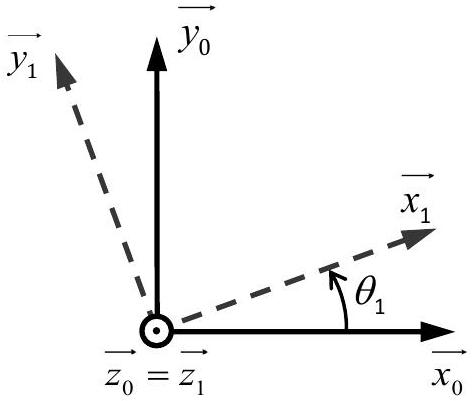
\includegraphics[max width=\textwidth, alt={}]{fa0d4e8b-3d38-4fa1-81c7-d2340e1d78c1-05_401_472_1789_414}
 & 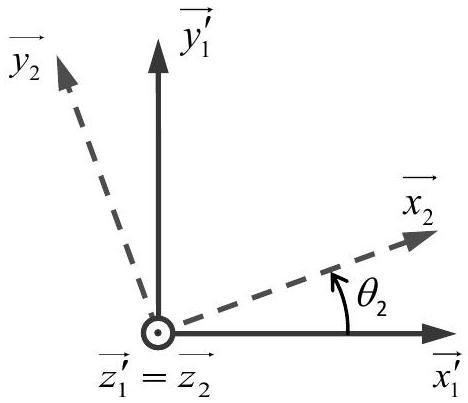
\includegraphics[max width=\textwidth, alt={}]{fa0d4e8b-3d38-4fa1-81c7-d2340e1d78c1-05_403_468_1787_924}
 & 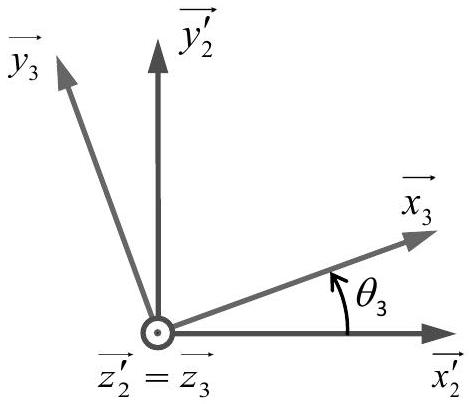
\includegraphics[max width=\textwidth, alt={}]{fa0d4e8b-3d38-4fa1-81c7-d2340e1d78c1-05_404_469_1787_1441}
 \\
\hline
Angles constants & 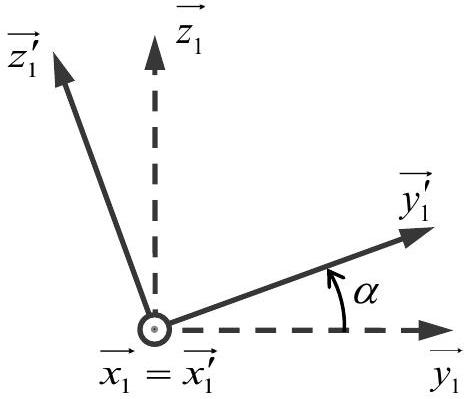
\includegraphics[max width=\textwidth, alt={}]{fa0d4e8b-3d38-4fa1-81c7-d2340e1d78c1-05_399_465_2242_416}
 & 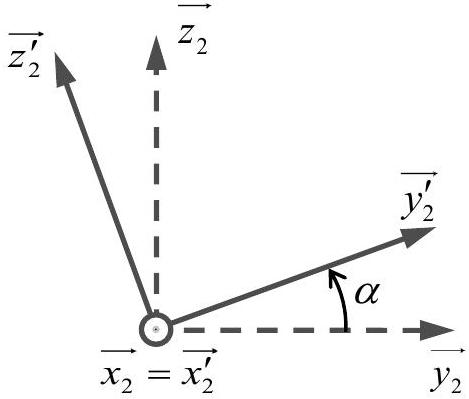
\includegraphics[max width=\textwidth, alt={}]{fa0d4e8b-3d38-4fa1-81c7-d2340e1d78c1-05_399_469_2242_926}
 & \( \begin{aligned} & \left(\overrightarrow{y_{1}}, \overrightarrow{y_{1}^{\prime}}\right)=\alpha=-22,5^{\circ} \\ & \left(\overrightarrow{y_{2}}, \overrightarrow{y_{2}^{\prime}}\right)=\alpha=-22,5^{\circ} \end{aligned} \) \\
\hline
\end{tabular}
\captionsetup{labelformat=empty}
\caption{Figure 6 - Figures de changement de base associées au robot porte-sonde}
\end{center}
\end{table}

\begin{itemize}
  \item[Q1.] En appliquant la loi de composition de mouvement sur les vecteurs vitesses au point $O$, montrer que $\overrightarrow{V_{S / 0}}\left(O_{S}\right)=\overrightarrow{0}$ avec la structure proposée.
  \item[Q2.] En appliquant la loi de composition de mouvement sur les vecteurs taux de rotation, justifier, sans développer les calculs, qu'il est a priori possible d'orienter le repère $\mathcal{R}_{3}$ lié à la sonde par rapport au repère $\mathcal{R}_{0}$, par 3 rotations suivant les vecteurs de la base $\left(\overrightarrow{x_{0}}, \overrightarrow{y_{0}}, \overrightarrow{z_{0}}\right)$.
  \item[Q3.] Conclure quant à la validation de l'exigence 1.1.1.
\end{itemize}

\section*{I. 2 - Validation de l'exigence " Espace de travail " (exigence 1.1.2)}
Objectif : vérifier l'étendue de l'espace de travail (exigence 1.1.2).\\
L'espace de travail d'un robot est défini comme l'ensemble des positions et orientations accessibles par le repère lié à son organe terminal. En se limitant à la configuration où la sonde reste en contact avec le patient (les points $O_{S}$ et $O$ restent confondus), la détermination de l'espace de travail revient ici à définir l'ensemble des orientations possibles pour l'ensemble \{porte-sonde, sonde\}, c'est-à-dire celles du repère $\mathcal{R}_{3}=\left(O, \overrightarrow{x_{3}}, \overrightarrow{y_{3}}, \overrightarrow{z_{3}}\right)$ par rapport au repère $\mathcal{R}_{0}=\left(O, \overrightarrow{x_{0}}, \overrightarrow{y_{0}}, \overrightarrow{z_{0}}\right)$.

\section*{Orientation de la sonde par rapport au patient}
À la sonde (S) est associé le repère $\mathcal{R}_{S}=\left(O_{S}, \overrightarrow{x_{S}}, \overrightarrow{y_{S}}, \overrightarrow{z_{S}}\right)$ défini sur la figure 7. Ce repère est coïncidant avec le repère $\mathcal{R}_{3}$. Le contact sonde/patient est assimilé à un contact ponctuel au point $O_{S}$. L'orientation de la sonde par rapport au patient est paramétrée par trois rotations successives $\mathrm{R}_{1}(\psi)$, $\mathrm{R}_{2}(\theta)$ et $\mathrm{R}_{3}(\phi)$ auxquelles sont associés les angles d'Euler $(\psi, \theta, \phi)$ (figures 7 et 8) :

\begin{itemize}
  \item[-] $\psi=\left(\overrightarrow{x_{0}}, \vec{u}\right)=\left(\overrightarrow{y_{0}}, \vec{v}\right)$ est associé à la rotation $\mathrm{R}_{1}$ autour de $\overrightarrow{\mathrm{z}_{0}}$ (précession);
  \item[-] $\theta=(\vec{v}, \vec{w})=\left(\overrightarrow{z_{0}}, \overrightarrow{z_{S}}\right)$ est associé à la rotation $\mathrm{R}_{2}$ autour du vecteur nodal $\overrightarrow{\mathrm{u}}$ (nutation);
  \item[-] $\phi=\left(\vec{u}, \overrightarrow{x_{S}}\right)=\left(\vec{w}, \overrightarrow{y_{S}}\right)$ est associé à la rotation $\mathrm{R}_{3}$ autour de $\overrightarrow{\mathrm{z}_{\mathrm{s}}}$ (rotation propre).
\end{itemize}

\begin{figure}[h]
\begin{center}
  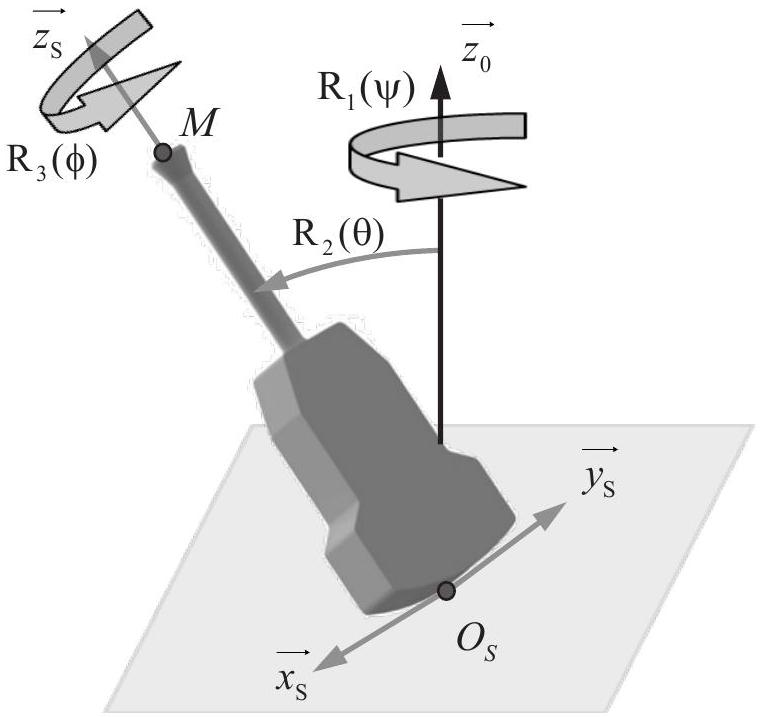
\includegraphics[alt={},max width=\textwidth]{fa0d4e8b-3d38-4fa1-81c7-d2340e1d78c1-06_717_762_1833_324}
\captionsetup{labelformat=empty}
\caption{Figure 7 - Repère lié à la sonde et rotations}
\end{center}
\end{figure}

\begin{figure}[h]
\begin{center}
  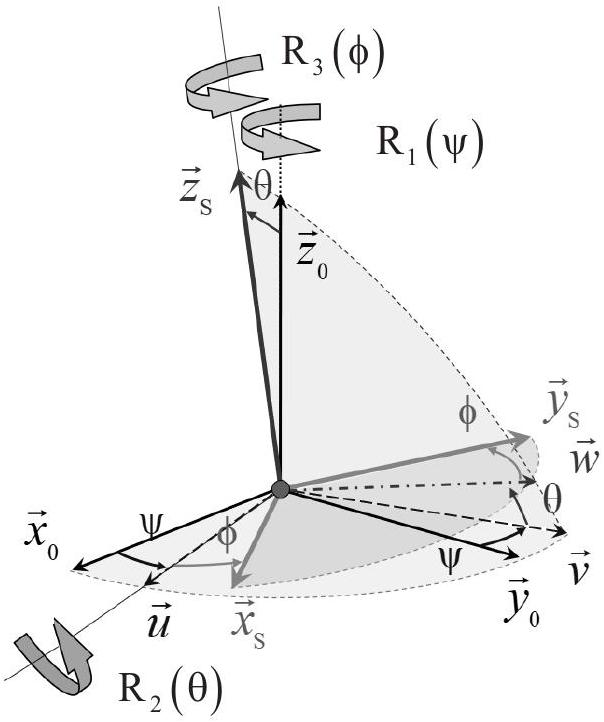
\includegraphics[alt={},max width=\textwidth]{fa0d4e8b-3d38-4fa1-81c7-d2340e1d78c1-06_722_604_1807_1230}
\captionsetup{labelformat=empty}
\caption{Figure 8 - Angles d'Euler}
\end{center}
\end{figure}

\section*{Élaboration d'un modèle géométrique direct partiel}
L'orientation de la sonde est paramétrée dans l'espace opérationnel (X) par les angles d'Euler $(\psi, \theta, \phi)$. Elle est liée à la configuration du robot définie quant à elle dans l'espace articulaire $(Q)$ par les angles $\left(\theta_{1}, \theta_{2}, \theta_{3}\right)$ paramétrant les rotations autour des axes 1, 2 et 3. La détermination de l'espace de travail nécessite d'établir la relation entre les coordonnées opérationnelles $(\psi, \theta, \phi)$ et les coordonnées articulaires $\left(\theta_{1}, \theta_{2}, \theta_{3}\right)$, c'est-à-dire élaborer le modèle géométrique direct du robot.

\begin{itemize}
  \item[Q4.] L'orientation de l'axe de la sonde étant définie par le vecteur $\overrightarrow{z_{S}}=\overrightarrow{z_{3}}$, déterminer les expressions des projections de ce vecteur dans la base $\left(\overrightarrow{x_{0}}, \overrightarrow{y_{0}}, \overrightarrow{z_{0}}\right)$, en fonction des coordonnées opérationnelles $(\psi, \theta)$.
\end{itemize}

De la même manière, il est possible d'exprimer ce vecteur en projection dans la base $\left(\overrightarrow{x_{0}}, \overrightarrow{y_{0}}, \overrightarrow{z_{0}}\right)$, en fonction des coordonnées articulaires $\left(\theta_{1}, \theta_{2}\right)$, ce qui conduit à :

$$
\overrightarrow{z_{3}}=\left(\begin{array}{c}
\cos \alpha \sin \alpha \sin \theta_{1}+\sin \alpha\left(\cos \alpha \sin \theta_{1} \cos \theta_{2}+\cos \theta_{1} \sin \theta_{2}\right) \\
-\cos \alpha \sin \alpha \cos \theta_{1}-\sin \alpha\left(\cos \alpha \cos \theta_{1} \cos \theta_{2}-\sin \theta_{1} \sin \theta_{2}\right) \\
\cos ^{2} \alpha-\sin ^{2} \alpha \cos \theta_{2}
\end{array}\right)_{\left(\overrightarrow{x_{0}}, \overrightarrow{y_{0}}, \overrightarrow{z_{0}}\right)} .
$$

\begin{itemize}
  \item[Q5.] Par identification des projections suivant $\overrightarrow{z_{0}}$, déterminer l'expression de l'angle de nutation $\theta$ en fonction des coordonnées articulaires. Commenter le résultat obtenu et proposer une analyse de la courbe donnée en figure 9.
  \item[Q6.] Montrer qu'en procédant de même avec les projections suivant $\overrightarrow{x_{0}}$ et $\overrightarrow{y_{0}}$, on obtient les expressions suivantes permettant de calculer l'angle de précession $\psi$ :
$$
\begin{aligned}
& \cos \psi=\frac{\sin \alpha\left(-\sin \theta_{1} \sin \theta_{2}+\cos \alpha \cos \theta_{1}\left(1+\cos \theta_{2}\right)\right)}{\sin \theta} \\
& \sin \psi=\frac{\sin \alpha\left(\cos \theta_{1} \sin \theta_{2}+\cos \alpha \sin \theta_{1}\left(1+\cos \theta_{2}\right)\right)}{\sin \theta} .
\end{aligned}
$$
\end{itemize}

Des relations similaires non présentées ici peuvent être obtenues pour la rotation propre $\phi$. L'ensemble de ces résultats permet notamment d'obtenir les courbes de la figure 10 qui représentent les évolutions des angles de précession et de rotation propre pour $\theta_{1}=0^{\circ}$ et $\theta_{2} \in\left[0^{\circ}, 180^{\circ}[\right.$.

\begin{itemize}
  \item[Q7.] À partir d'une analyse des courbes obtenues, préciser en justifiant la réponse :
  \begin{itemize}
    \item[a)] les configurations dans lesquelles se trouve le robot pour les valeurs extrêmes de l'angle de nutation $\theta$ relatives à la courbe de la figure 9 ;
    \item[b)] les valeurs associées de l'angle $\beta=\left(\overrightarrow{x_{0}}, \overrightarrow{x_{S}}\right)$;
    \item[c)] la nature et les caractéristiques de la surface générée par le mouvement de l'axe de la sonde $\left(O, \overrightarrow{z_{S}}\right)$.
  \end{itemize}
  \item[Q8.] En considérant les rotations suivant les axes $1\left(\theta_{1} \in\left[-180^{\circ}, 180^{\circ}\right]\right)$ et $3\left(\theta_{3} \in\left[0^{\circ}, 360^{\circ}\right]\right)$, conclure quant à l'ensemble des orientations théoriquement possibles pour la sonde.
\end{itemize}

\begin{figure}[h]
\begin{center}
  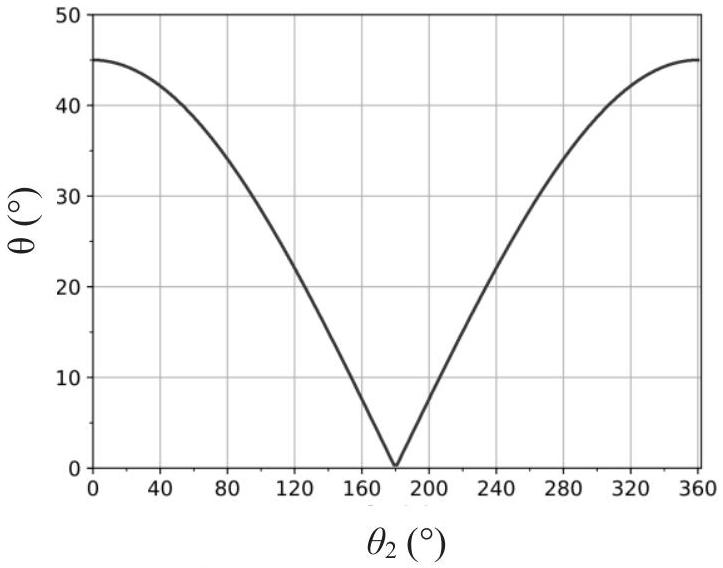
\includegraphics[alt={},max width=\textwidth]{fa0d4e8b-3d38-4fa1-81c7-d2340e1d78c1-08_568_723_178_250}
\captionsetup{labelformat=empty}
\caption{Figure 9 - Évolution de l'angle de nutation $\theta$ en fonction du paramètre articulaire $\theta_{2}$}
\end{center}
\end{figure}

\begin{figure}[h]
\begin{center}
  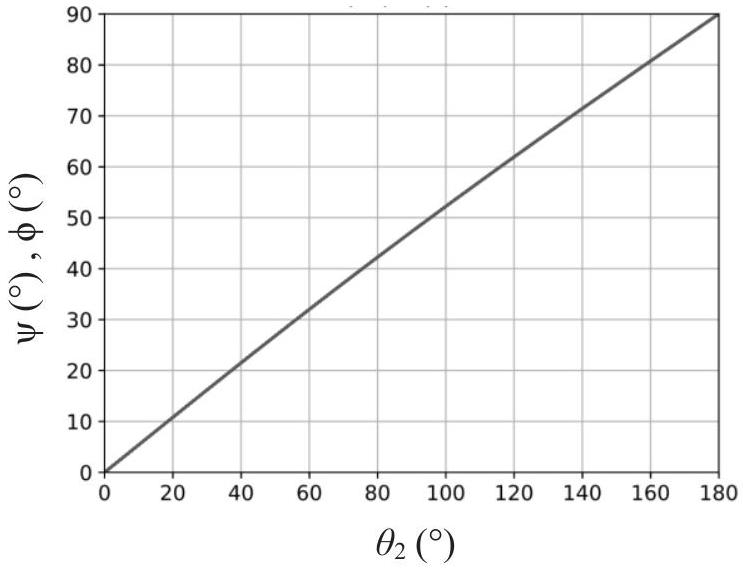
\includegraphics[alt={},max width=\textwidth]{fa0d4e8b-3d38-4fa1-81c7-d2340e1d78c1-08_568_743_178_1049}
\captionsetup{labelformat=empty}
\caption{Figure 10 - Évolution des angles $\psi$ et $\phi$ (les courbes sont ici confondues)}
\end{center}
\end{figure}

\section*{Prise en compte des butées articulaires}
En pratique, l'espace de travail est limité par la présence de butées mécaniques sur les articulations, liées aux contraintes de mise en œuvre technique. En prenant comme référence la position du robot " bras tendu ", les valeurs de ces butées sont telles que pour les deux premiers axes : $\theta_{1} \in\left[-165^{\circ}, 165^{\circ}\right], \theta_{2} \in\left[20^{\circ}, 340^{\circ}\right]$. Il n'y a pas de limitation sur l'axe 3 pour lequel $\theta_{3} \in\left[0^{\circ}, 360^{\circ}\right]$. L'espace de travail peut être décrit à partir des positions accessibles par le point $M$, extrémité du vecteur unitaire $\overrightarrow{z_{S}}$ d'origine $O_{S}$, porté par l'axe de la sonde (figure 7). Les points de coordonnées $\left(z_{S x}, z_{S y}, z_{S z}\right)$ associés à ces positions ont été représentés sur la figure 11 (le pas d'échantillonnage des paramètres articulaires $\theta_{1}$ et $\theta_{2}$ est de 2°) pour deux configurations (a) et (b).

\begin{figure}[h]
\begin{center}
  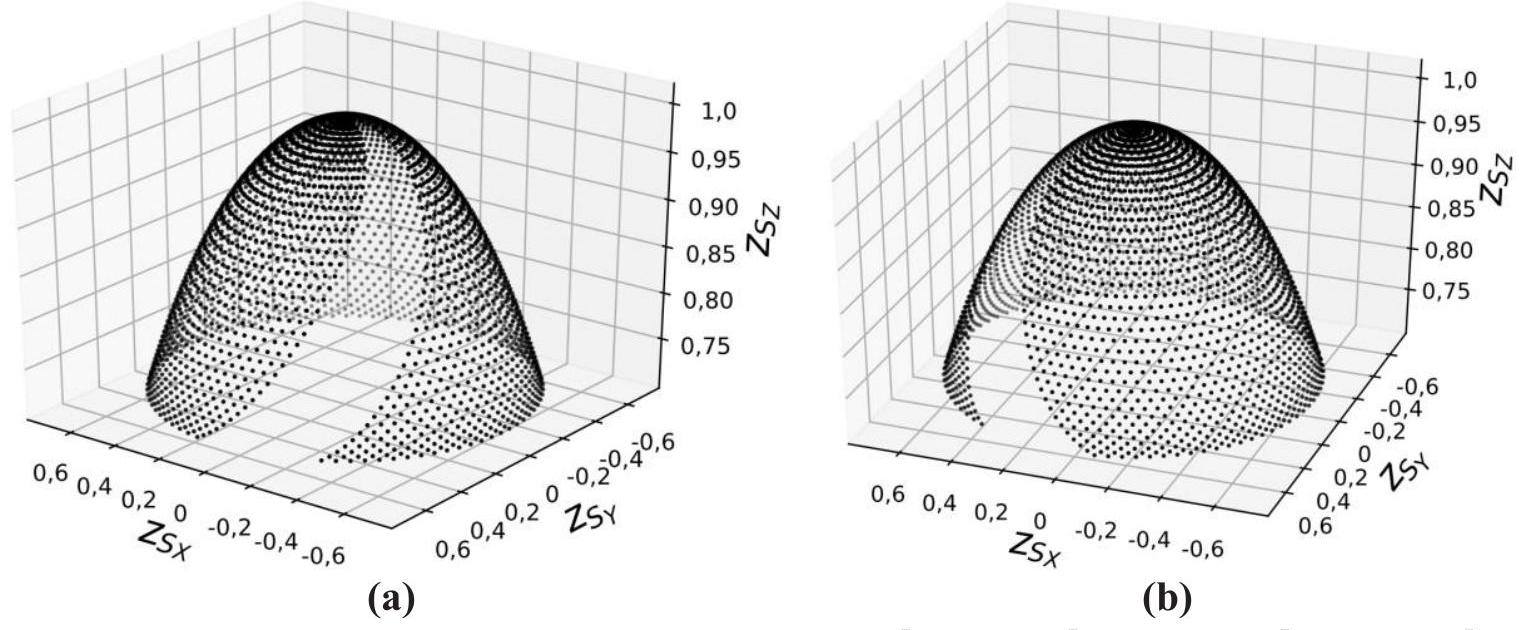
\includegraphics[alt={},max width=\textwidth]{fa0d4e8b-3d38-4fa1-81c7-d2340e1d78c1-08_630_1529_1493_272}
\captionsetup{labelformat=empty}
\caption{Figure 11 - Représentation de l'espace de travail, $\theta_{2} \in\left[20^{\circ}, 180^{\circ}\right]$ (a) et $\theta_{2} \in\left[180^{\circ}, 340^{\circ}\right]$ (b)}
\end{center}
\end{figure}

\begin{itemize}
  \item[Q9.] À partir de l'analyse des tracés de la figure 11, conclure quant à la validation de l'exigence 1.1.2, liée à l'espace de travail attendu.
\end{itemize}

Soit la fonction $f$, définie de l'espace articulaire $(Q)$ vers l'espace opérationnel $(\mathrm{X})$, dont les applications coordonnées ( $f_{1}, f_{2}$ ) sont telles que $f_{1}\left(\theta_{1}, \theta_{2}\right)=\theta$ et $f_{2}\left(\theta_{1}, \theta_{2}\right)=\psi$.

\begin{itemize}
  \item[Q10.] La fonction $f$ est-elle bijective ? Justifier votre réponse en vous appuyant sur les tracés de la figure 11 et proposer une interprétation. Quelles seront les conséquences lors de la conception de la commande du robot ?
\end{itemize}

\section*{Partie II - Commande en position du robot porte-sonde}
Objectif : vérifier que les différentes exigences 1.2 relatives à la commande en position du robot porte-sonde peuvent être satisfaites.

\section*{II. 1 - Principe de la commande du robot porte-sonde}
La commande du robot porte-sonde repose sur la mise en œuvre de deux couches matérielles et logicielles qui communiquent l'une avec l'autre (figure 12).

\begin{itemize}
  \item[-] Le contrôleur haut niveau, implémenté sur le PC de contrôle du poste patient, reçoit en paramètres d'entrée, les coordonnées du positionnement désiré pour la sonde échographique, dans l'espace de travail (précession $\psi$, nutation $\theta$, rotation propre $\varphi$ ) ainsi que les positions articulaires $\left(\theta_{1}, \theta_{2}, \theta_{3}\right)$ acquises par le contrôle bas-niveau. L'ensemble de ces données est traité numériquement (calcul des modèles géométriques direct et inverse du robot, prise en compte des butées articulaires, des changements d'aspect et le traitement des singularités) afin de déterminer les consignes articulaires à transmettre au contrôleur bas niveau.
  \item[-] Le contrôleur bas niveau, implémenté sur la carte d'axes, reçoit les consignes articulaires et calcule les profils de vitesse $\left(\omega_{1}(\mathrm{t}), \omega_{2}(\mathrm{t}), \omega_{3}(\mathrm{t})\right)$ transmis ensuite aux variateurs de vitesse qui pilotent les moteurs des différents axes du robot. Il assure également l'acquisition des positions articulaires qui sont communiquées au contrôleur haut niveau.
\end{itemize}

\begin{figure}[h]
\begin{center}
  \includegraphics[alt={},max width=\textwidth]{fa0d4e8b-3d38-4fa1-81c7-d2340e1d78c1-09_267_1439_1223_302}
\captionsetup{labelformat=empty}
\caption{Figure 12 - Principe de la commande du robot porte-sonde}
\end{center}
\end{figure}

\section*{Commande de l'axe 1}
On se limite ici à l'étude de la commande du premier axe, dont la structure est présentée en figure 4. Le principe associé à cette commande est décrit par la figure 13. La structure de commande de la position angulaire $\theta_{1}$ est composée de deux boucles imbriquées disposant chacune d'un réseau correcteur :

\begin{itemize}
  \item[-] une boucle interne de vitesse, gérée par le variateur ;
  \item[-] une boucle externe de position, gérée par la carte d'axes.
\end{itemize}

Un codeur incrémental, solidaire de l'axe moteur permet après traitement numérique d'obtenir une image de la position angulaire $\theta_{1}$ et de la vitesse angulaire $\omega_{1}$ de l'axe 1, grandeurs mises en œuvre au niveau des deux boucles d'asservissement. La consigne de position est élaborée par la carte d'axes, par intégration du profil de vitesse généré.

\begin{figure}[h]
\begin{center}
  \includegraphics[alt={},max width=\textwidth]{fa0d4e8b-3d38-4fa1-81c7-d2340e1d78c1-09_297_1476_2248_289}
\captionsetup{labelformat=empty}
\caption{Figure 13 - Structure de l'asservissement d'un axe}
\end{center}
\end{figure}

\section*{II. 2 - Modélisation de l'axe 1}
Objectif : élaborer un modèle de connaissance de l'axe 1 et réaliser la synthèse de la commande.

\section*{Modélisation de la motorisation}
La motorisation de l'axe 1 est réalisée à l'aide d'un moteur électrique à courant continu et aimants permanents, dont le comportement peut être modélisé par les équations suivantes :


\begin{align*}
& u(t)=R i(t)+L \frac{d i(t)}{d t}+e(t)  \tag{1}\\
& e(t)=k_{e} \omega_{m}(t) \tag{2}
\end{align*}



\begin{align*}
& C_{m}(t)=k_{c} i(t) \\
& C_{m}(t)-C_{r e}(t)=J_{e q} \frac{d \omega_{m}(t)}{d t} \tag{4}
\end{align*}


Les différentes grandeurs intervenant dans le modèle sont définies dans le tableau 2 suivant :

\begin{table}[h]
\begin{center}
\begin{tabular}[t]{|l|l|l|}
\hline
Symbole & Désignation & Unités / valeurs \\
\hline
$u(t)$ & Tension d'induit & V \\
\hline
$e(t)$ & Force contre-électromotrice & V \\
\hline
$i(t)$ & Courant d'induit & A \\
\hline
$\omega_{m}(t)$ & Vitesse de rotation du moteur & rad/s \\
\hline
$C_{m}(t)$ & Couple moteur & $\mathrm{N} \cdot \mathrm{m}$ \\
\hline
$C_{\text {re }}(t)$ & Couple résistant équivalent ramené sur l'axe moteur & $\mathrm{N} \cdot \mathrm{m}$ \\
\hline
$R$ & Résistance de l'induit & $4,1 \Omega$ \\
\hline
$L$ & Inductance de l'induit & $0,18 \mathrm{mH}$ \\
\hline
$k_{e}$ & Constante de force contre-électromotrice & $1,6 \cdot 10^{-2} \mathrm{~V} /(\mathrm{rad} / \mathrm{s})$ \\
\hline
$k_{c}$ & Constante de couple & $1,6 \cdot 10^{-2} \mathrm{~N} \cdot \mathrm{~m} / \mathrm{A}$ \\
\hline
$J_{\text {eq }}$ & Inertie équivalente ramenée sur l'axe moteur & $\in\left[7,2 \cdot 10^{-6}, 8,6 \cdot 10^{-6}\right] \mathrm{kg} \cdot \mathrm{m}^{2}$ \\
\hline
\end{tabular}
\captionsetup{labelformat=empty}
\caption{Tableau 2 - Grandeurs associées au modèle de la motorisation}
\end{center}
\end{table}

On note $\Omega_{m}(p), U(p), E(p), I(p), C_{m}(p)$ et $C_{r e}(p)$, les transformées de Laplace respectives de $\omega_{m}(\mathrm{t}), u(t), e(t), i(t), C_{m}(t)$ et $C_{\text {re }}(t)$.

\begin{itemize}
  \item[Q11.] Déterminer sur la copie les transformées de Laplace des équations (1) à (4) du moteur définies en considérant des conditions initiales nulles. Compléter les blocs correspondants sur le schéma bloc du Document Réponse DR1 par les transmittances manquantes.
  \item[Q12.] Déterminer les expressions littérales des fonctions de transfert en suivi de consigne $H_{1}(p)=\left.\frac{\Omega_{m}(p)}{U(p)}\right|_{C_{r e}(p)=0}$ et en régulation $H_{2}(p)=\left.\frac{\Omega_{m}(p)}{C_{r e}(p)}\right|_{U(p)=0}$, sous forme canonique.
\end{itemize}

On pose $\tau_{e}=\frac{L}{R}$ et $\tau_{e m}=\frac{R J_{e q}}{k_{e} k_{c}}$, respectivement constantes de temps électrique et électromécanique du moteur à courant continu.

\begin{itemize}
  \item[Q13.] Déterminer les valeurs numériques des constantes de temps $\tau_{e}$ et $\tau_{e m}$, pour les valeurs extrêmes de $J_{e q}$. En déduire qu'une constante de temps peut être considérée comme négligeable devant l'autre.
  \item[Q14.] Montrer, en précisant l'expression de $K_{m}$, que la fonction $H_{1}(p)$ peut alors être approximée par la forme : $H_{1}(p) \approx \frac{K_{m}}{\left(1+\tau_{e} p\right)\left(1+\tau_{e m} p\right)}$.
\end{itemize}

\section*{Modélisation de la boucle de vitesse}
La figure 14 présente la structure de la boucle de vitesse associée à la commande de l'axe 1. Pour une consigne de vitesse de rotation $\omega_{\mathrm{c}}(\mathrm{t})$ [m/s], un convertisseur génère une tension de consigne de rotation à appliquer au moteur $\mathrm{u}_{\mathrm{cv}}(\mathrm{t})[\mathrm{V}]$. Un traitement numérique de la vitesse relevée sur l'axe du moteur fournit une tension mesurée $\mathrm{u}_{\mathrm{mv}}(\mathrm{t})$ [V], image de la vitesse de rotation du moteur $\omega_{\mathrm{m}}(\mathrm{t})$. Un correcteur adapte le signal écart entre la tension de consigne et la tension mesurée, ce qui permet après correction et amplification, de définir la tension d'alimentation $\mathrm{u}_{\mathrm{m}}(\mathrm{t})$ à appliquer au moteur.

\begin{figure}[h]
\begin{center}
  \includegraphics[alt={},max width=\textwidth]{fa0d4e8b-3d38-4fa1-81c7-d2340e1d78c1-11_393_1668_1048_224}
\captionsetup{labelformat=empty}
\caption{Figure 14 - Asservissement en vitesse d'un axe}
\end{center}
\end{figure}

Le tableau 3 liste les gains des différents composants intervenant dans la commande de l'axe 1.

\begin{table}[h]
\begin{center}
\begin{tabular}[t]{|l|l|}
\hline
Blocs & Fonctions de transfert \\
\hline
Convertisseur & $K_{\text {conv }}$ (à déterminer) \\
\hline
Correcteur vitesse & $C_{V}(p)$ (réglé par la suite) \\
\hline
Amplificateur/variateur & $K_{A}=9,4$ \\
\hline
Codeur et traitement & $K_{\text {vit }}=8,3 \cdot 10^{-3} \mathrm{~V} /(\mathrm{rad} / \mathrm{s})$ \\
\hline
Réducteurs & $K_{R}$ (à déterminer) \\
\hline
\end{tabular}
\captionsetup{labelformat=empty}
\caption{Tableau 3 - Fonctions associées aux blocs du modèle}
\end{center}
\end{table}

On rappelle que les caractéristiques de la transmission sont définies dans le tableau 1.

\begin{itemize}
  \item[Q15.] Déterminer les expressions des gains $K_{R}$ et $K_{\text {conv }}$ ainsi que les valeurs numériques et unités associées.
  \item[Q16.] Compléter le schéma-bloc sur le DR 1 en y faisant figurer les fonctions de transfert sous forme littérale dans le domaine de Laplace avec des conditions initiales nulles.
\end{itemize}

On pourrait montrer que le schéma-bloc peut se ramener au schéma à retour unitaire de la figure 15, avec $G_{1}(p)=\frac{k_{c}}{R} \cdot \frac{1}{1+\tau_{e} p}, G_{2}(p)=\frac{R}{k_{c}} \cdot \frac{1}{1+\tau_{e m} p}$ et $K=K_{v i t} K_{A} K_{m}$.

\begin{itemize}
  \item[Q17.] À partir du schéma-bloc à retour unitaire de la figure 15, déterminer l'expression de la fonction de transfert en boucle ouverte $H_{B O}(p)=\frac{\Omega_{s}(p)}{\varepsilon_{V}(p)}$, en fonction de $C_{V}(p), \tau_{e}, \tau_{e m}$, et $K$.
\end{itemize}

\begin{figure}[h]
\begin{center}
  \includegraphics[alt={},max width=\textwidth]{fa0d4e8b-3d38-4fa1-81c7-d2340e1d78c1-12_338_1555_339_248}
\captionsetup{labelformat=empty}
\caption{Figure 15 - Schéma-bloc équivalent pour la boucle de vitesse}
\end{center}
\end{figure}

\begin{itemize}
  \item[Q18.] En vous appuyant sur le schéma-bloc de la figure 15 et sur une analyse de la fonction de transfert $H_{B O}(p)$, discuter de la validation de l'exigence 1.2.1.1.2. Conclure sur la nécessité de mettre en place une action intégrale au niveau du correcteur.
\end{itemize}

\section*{II. 3 - Synthèse de la commande : boucle de vitesse}
Objectif : déterminer les paramètres du correcteur de la boucle de vitesse afin de satisfaire l'exigence 1.2.1.1.

Le système est à présent considéré en l'absence de perturbation (étude en suivi de consigne), soit $C_{r e}(p)=0$. Le correcteur de la boucle de vitesse est un correcteur Proportionnel Intégral (PI), de fonction de transfert :

$$
C_{V}(p)=K_{i} \frac{1+T_{i} p}{T_{i} p} .
$$

La constante de temps $T_{i}$ est choisie de manière à compenser le pôle dominant de la fonction de transfert du moteur, ce qui revient ici à prendre $T_{i}=\tau_{e m}$.

\begin{itemize}
  \item[Q19.] Déterminer, en fonction des paramètres $K_{i}, K, \tau_{e m}$ et $\tau_{e}$, l'expression littérale de la fonction de transfert en vitesse sous la forme canonique d'un système du second ordre
$$
H_{V}(p)=\frac{\Omega_{s}(p)}{\Omega_{c}(p)}=\frac{K_{V}}{1+\frac{2 z}{\omega_{0}} p+\frac{1}{\omega_{0}^{2}} p^{2}} .
$$
Préciser la valeur de $K_{V}$ et les expressions littérales de $z$ et $\omega_{0}$.
\end{itemize}

Le gain $K_{i}$ du correcteur est fixé de manière à obtenir la réponse la plus rapide sans dépassement en boucle fermée. On rappelle que pour un modèle du second ordre, la réponse la plus rapide sans dépassement est obtenue pour un facteur d'amortissement $z=1$, valeur pour laquelle on a $t_{r 5 \%} \cdot \omega_{0} \approx 5$. On se place dans le cas où l'inertie équivalente est maximale, soit $J_{e q}=8,6 \cdot 10^{-6} \mathrm{~kg} \cdot \mathrm{~m}^{2}$.

\begin{itemize}
  \item[Q20.] Déterminer l'expression de $K_{i}$ ainsi que sa valeur numérique. Déterminer la valeur du temps de réponse $t_{r 5 \%}$ de la boucle de vitesse pour cette valeur de $K_{i}$.
\end{itemize}

On donne, sur le DR 2, le diagramme de Bode de la fonction de transfert en boucle ouverte du système ainsi corrigé.

\begin{itemize}
  \item[Q21.] Sur le DR 2, déterminer graphiquement les marges de stabilité du système et préciser leurs valeurs.
\end{itemize}

\section*{Prise en compte des non-linéarités dans la commande : " synthèse "}
On souhaite simuler la réponse en vitesse de l'axe 1 en intégrant dans le modèle certaines nonlinéarités : le variateur délivre une tension comprise entre $\pm 10 \mathrm{~V}$ et le courant moteur est limité à 5A. À cet effet, on construit le modèle numérique présenté en figure 16.

\begin{figure}[h]
\begin{center}
  \includegraphics[alt={},max width=\textwidth]{fa0d4e8b-3d38-4fa1-81c7-d2340e1d78c1-13_458_1687_685_192}
\captionsetup{labelformat=empty}
\caption{Figure 16 - Modèle numérique utilisé pour la simulation de la boucle de vitesse}
\end{center}
\end{figure}

Les courbes du DR 3 présentent les réponses en vitesse de l'axe 1, pour une entrée en échelon d'amplitude 0,1 rad/s ainsi que l'évolution de la tension aux bornes du moteur, sans et avec prise en compte de ces non-linéarités.

\begin{itemize}
  \item[Q22.] Sur le DR 3, identifier les courbes correspondant aux simulations sans et avec prise en compte des non-linéarités. Commenter, sur la copie, l'évolution des performances en termes de rapidité.
  \item[Q23.] En exploitant les résultats précédents, proposer, sous forme de tableau, une synthèse des exigences de performances associées à la boucle de vitesse. Conclure quant à la validation de l'exigence 1.2.1.1.
\end{itemize}

\section*{II. 4 - Performances de la commande en position}
Objectif : vérifier les performances attendues pour la boucle de position (exigence 1.2.1.2.).\\
Les performances de la boucle de vitesse étant validées, on complète le modèle numérique avec la boucle de position (figure 13). Les paramètres du correcteur Proportionnel Intégral Dérivé (PID) de la boucle de position sont déterminés à l'aide de l'outil de simulation numérique. La réponse temporelle en position de l'axe 1, pour une consigne en échelon de 10°, est représentée sur la figure du DR 4.

\begin{itemize}
  \item[Q24.] En faisant apparaître les constructions, déterminer graphiquement sur le DR 4 le temps de réponse à 5\% du système. Conclure quant au respect de l'exigence 1.2.1.2.
\end{itemize}

\section*{Partie III - Dimensionnement du moteur d'axe 1}
Objectif : déterminer le couple moteur nécessaire à l'entraînement en rotation autour de l'axe 1.\\
Le robot se trouvant dans la configuration bras tendu représenté sur la figure 17, on étudie la rotation $\mathrm{R}_{1}$ autour de l'axe $1\left(A, \vec{z}_{1}\right)$. Les trois autres degrés de liberté (rotations $\mathrm{R}_{2}$ et $\mathrm{R}_{3}$, translation T) du robot sont bloqués, de telle sorte que $\theta_{2}(t)=0, \theta_{3}(t)=0$ et l'extrémité de la sonde reste confondue avec l'origine $O$. La définition des solides, repères et angles, est celle proposée pour l'étude cinématique (figures 5 et 6), complétée ici avec le groupe de motorisation de l'axe 1, constitué du moteur (stator lié à 1 et rotor), du réducteur et de la transmission poulies-courroie.

Afin de déterminer le couple moteur nécessaire pour réaliser l'entraînement en rotation autour de l'axe $1\left(A, \vec{z}_{1}\right)$, on propose d'appliquer le théorème de l'énergie cinétique à l'ensemble en mouvement par rapport à $\mathbf{0}$. Le référentiel auquel est associé le repère $\mathcal{R}_{0}\left(O, \overrightarrow{x_{0}}, \overrightarrow{y_{0}}, \overrightarrow{z_{0}}\right)$ est considéré comme Galiléen.

On note :

\begin{itemize}
  \item[-] $\boldsymbol{E}_{1}^{\prime}$, l'ensemble constitué des solides 1, 2, 3, 4 et du stator moteur ;
  \item[-] $\boldsymbol{E}_{5}$, l'ensemble constitué du rotor, des parties mobiles du réducteur et de la poulie $\mathrm{P}_{1}$.
\end{itemize}

Le système est soumis aux actions mécaniques extérieures suivantes :

\begin{itemize}
  \item[-] action de la pesanteur : $\left\{\tau_{\text {pes } \rightarrow E_{1}^{\prime}}\right\}=\left\{\begin{array}{c}-m_{1} g \overrightarrow{z_{0}} \\ \overrightarrow{0}\end{array}\right\}_{G_{1}}$ et $\left\{\tau_{\text {pes } \rightarrow E_{5}}\right\}=\left\{\begin{array}{c}-m_{5} g \overrightarrow{z_{0}} \\ \overrightarrow{0}\end{array}\right\}_{G_{5}}$;
  \item[-] action associée au contact sonde/patient : $\left\{\tau_{0 \rightarrow 4}\right\}=\left\{\begin{array}{c}F_{C} \overrightarrow{z_{3}} \\ C_{R} \overrightarrow{y_{3}}+C_{P} \overrightarrow{z_{3}}\end{array}\right\}_{O}$.
\end{itemize}

L'action d'entraînement du rotor moteur par le stator, considérée ici comme une action mécanique intérieure, est modélisée par le torseur suivant : $\left\{\tau_{\text {Stator } \rightarrow \text { Rotor }}\right\}=\left\{\begin{array}{c}\overrightarrow{0} \\ C_{m} \overrightarrow{z_{1}}\end{array}\right\}_{\forall P \in\left(D, \overrightarrow{z_{1}}\right)}$.

Les liaisons sont supposées sans frottement et la transmission de puissance par le système pouliescourroie s'effectue sans glissement.

Paramétrage cinématique

\begin{itemize}
  \item[-] $\mathcal{R}_{1}\left(A, \overrightarrow{x_{1}}, \overrightarrow{y_{1}}, \overrightarrow{z_{1}}\right)$ est le repère associé à l'ensemble $\boldsymbol{E}_{1}^{\prime}$;\\
La rotation de $\boldsymbol{E}_{1}^{\prime} / \mathbf{0}$ est paramétrée par l'angle variable $\theta_{1}(t)=\left(\overrightarrow{x_{0}}, \overrightarrow{x_{1}}\right)=\left(\overrightarrow{y_{0}}, \overrightarrow{y_{1}}\right)$.
  \item[-] $\mathcal{R}_{5}\left(D, \overrightarrow{x_{5}}, \overrightarrow{y_{5}}, \overrightarrow{z_{5}}\right)$ est le repère associé à l'arbre de sortie du réducteur ;\\
La rotation de $\mathcal{R}_{5} / \mathcal{R}_{1}$ est paramétrée par l'angle variable $\theta_{5}(t)=\left(\overrightarrow{x_{1}}, \overrightarrow{x_{5}}\right)=\left(\overrightarrow{y_{1}}, \overrightarrow{y_{5}}\right)$.
  \item[-] $\mathcal{R}_{\mathrm{m}}\left(D, \overrightarrow{x_{\mathrm{m}}}, \overrightarrow{y_{\mathrm{m}}}, \overrightarrow{z_{5}}\right)$ est le repère associé au rotor moteur ;\\
La rotation de $\mathcal{R}_{\mathrm{m}} / \mathcal{R}_{1}$ est paramétrée par l'angle variable $\theta_{m}(t)=\left(\overrightarrow{x_{1}}, \overrightarrow{x_{\mathrm{m}}}\right)=\left(\overrightarrow{y_{1}}, \overrightarrow{y_{\mathrm{m}}}\right)$.
\end{itemize}

\section*{Données cinétiques}
Ensemble $\boldsymbol{E}_{1}^{\prime}=\{\mathbf{1 , 2 , 3 , 4 , \text { stator } \}}$

\begin{itemize}
  \item[-] $m_{1}$ : masse de l'ensemble $\boldsymbol{E}_{1}^{\prime}$;
  \item[-] $G_{1}$ : centre d'inertie de l'ensemble $\boldsymbol{E}_{1}^{\prime}$ tel que $\overrightarrow{A G_{1}}=y_{1} \overrightarrow{y_{1}}-z_{1} \overrightarrow{z_{1}}$;
  \item[-] $\overline{\bar{I}}\left(E_{1}^{\prime}, G_{1}\right)$ : matrice d'inertie dans la base $B_{1}$ au point $G_{1}$ telle que :
$$
\overline{\bar{I}}\left(E_{1}^{\prime}, G_{1}\right)=\left[\begin{array}{ccc}
A_{1} & 0 & 0 \\
0 & B_{1} & -D_{1} \\
0 & -D_{1} & C_{1}
\end{array}\right]_{B_{1}} .
$$
\end{itemize}

Ensemble $\boldsymbol{E}_{5}=\{$ rotor , réducteur, poulie $\}$

\begin{itemize}
  \item[-] $m_{5}$ : masse de l'ensemble $\boldsymbol{E}_{5}$;
  \item[-] $G_{5}$ : centre d'inertie de l'ensemble $\boldsymbol{E}_{5}$ situé sur l'axe $\left(D, \overrightarrow{z_{5}}\right)$ et tel que $\overrightarrow{A G_{5}}=-y_{5} \overrightarrow{y_{1}}-z_{5} \overrightarrow{z_{1}}$;
  \item[-] $I_{5}$ : moment d'inertie équivalent de l'ensemble $\boldsymbol{E}_{5}$ ramené au rotor moteur.
\end{itemize}

\begin{figure}[h]
\begin{center}
  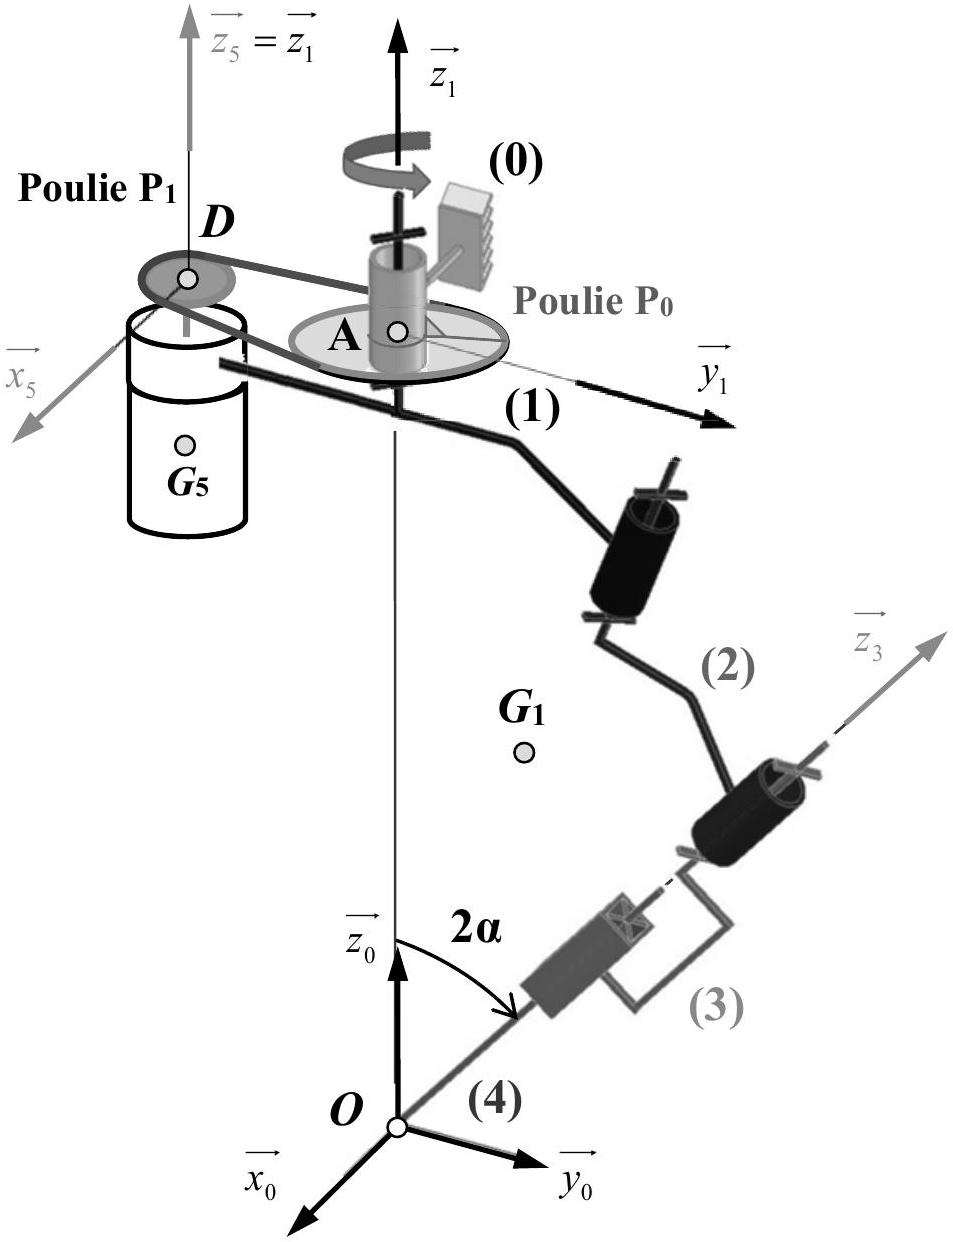
\includegraphics[alt={},max width=\textwidth]{fa0d4e8b-3d38-4fa1-81c7-d2340e1d78c1-15_1242_953_159_926}
\captionsetup{labelformat=empty}
\caption{Figure 17 - Schéma cinématique et paramétrage retenus pour le dimensionnement du moteur d'axe 1}
\end{center}
\end{figure}

\section*{Détermination de l'énergie cinétique du système}
\begin{itemize}
  \item[Q25.] Préciser les hypothèses qui ont conduit à considérer une matrice d'inertie sous la forme proposée pour l'ensemble $\boldsymbol{E}_{1}^{\prime}$.
  \item[Q26.] Déterminer l'expression de l'énergie cinétique galiléenne $E_{C}\left(\boldsymbol{E}_{1}^{\prime} / 0\right)$ de l'ensemble $\boldsymbol{E}_{1}^{\prime}$ en fonction du paramètre de mouvement $\dot{\theta}_{1}(t)$.
\end{itemize}

La détermination de l'énergie cinétique pour l'ensemble $\boldsymbol{E}_{5}$ conduirait à :

$$
E_{C}\left(E_{5} / 0\right)=\frac{1}{2} m_{5} y_{5}^{2} \dot{\theta}_{1}^{2}+\frac{1}{2} I_{5}\left(\dot{\theta}_{m}+\dot{\theta}_{1}\right)^{2} .
$$

Une étude cinématique de la transmission réalisée par le réducteur et l'ensemble poulies-courroie, dont les caractéristiques sont précisées par la figure 3, permettrait d'établir la relation suivante :

$$
\dot{\theta}_{1}(t)=-\frac{D_{1}}{D_{0}} r \dot{\theta}_{m}(t) .
$$

\begin{itemize}
  \item[Q27.] Donner alors l'expression de l'énergie cinétique totale $E_{C}\left(\left\{E_{1}^{\prime}+E_{5}\right\} / 0\right)$ en fonction du seul paramètre de mouvement $\dot{\theta}_{1}(t)$. En déduire l'expression du moment d'inertie équivalent $J_{1}$ ramené à l'axe $1\left(A, \vec{z}_{1}\right)$.
\end{itemize}

Détermination des puissances extérieures et intérieures\\
Q28. Déterminer les expressions des différentes puissances extérieures au système en fonction du seul paramètre $\dot{\theta}_{1}(t)$; on rappelle que dans la configuration étudiée $\theta_{2}(t)=0, \theta_{3}(t)=0$.

Q29. Déterminer l'expression de la puissance intérieure en fonction du seul paramètre $\dot{\theta}_{1}(t)$.

Application du théorème de l'énergie cinétique et détermination du couple moteur\\
Q30. Déterminer l'expression du couple moteur $C_{m}$ en appliquant le théorème de l'énergie cinétique. On donne les valeurs numériques suivantes pour une valeur de $\dot{\theta}_{1}$ donnée :

$$
J_{1}=9,9 \cdot 10^{-3} \mathrm{~kg} \cdot \mathrm{~m}^{2}, C_{R}=-2 \cdot 10^{-2} \mathrm{~N} \cdot \mathrm{~m}, C_{P}=-1 \cdot 10^{-1} \mathrm{~N} \cdot \mathrm{~m} .
$$

Q31. Déterminer la valeur numérique du couple moteur maximal $C_{\text {Max }}$ lorsque $\ddot{\theta}_{1}=7 \mathrm{rad} \cdot \mathrm{s}^{-2}$.

\section*{Partie IV - Analyse du geste médical (Informatique pour tous)}
Les questions d'informatique doivent être traitées en langage Python.\\
Objectif : spécifier les exigences 1.1 relatives au déplacement de la sonde.\\
Afin de définir certaines caractéristiques du mouvement que devra imposer le robot porte-sonde à la sonde échographique, il est nécessaire de procéder à une analyse du geste médical. Pour cela, la sonde est équipée d'un dispositif de localisation magnétique permettant de réaliser des mesures de position et d'orientation au cours d'un examen échographique classique.

Lorsque la sonde est en position initiale sur le patient, le repère sonde $\mathcal{R}_{S}=\left(O_{S}, \overrightarrow{x_{S}}, \overrightarrow{y_{S}}, \overrightarrow{z_{S}}\right)$ défini sur la figure 7 coïncide avec le repère de référence $\mathcal{R}_{0}=\left(O, \overrightarrow{x_{0}}, \overrightarrow{y_{0}}, \overrightarrow{z_{0}}\right)$ lié au patient. Comme illustré sur la figure 18, l'évolution de l'inclinaison de l'axe de la sonde au cours de l'examen est caractérisée en relevant la trajectoire du projeté de l'extrémité du vecteur unitaire $\overrightarrow{z_{s}}$ d'origine $O$ porté par l'axe de la sonde dans un plan $\left(P_{0}, \overrightarrow{x_{0}}, \overrightarrow{y_{0}}\right)$.\\
La trajectoire $P_{0} P$ peut être décrite à partir des composantes $z_{S x}=\overrightarrow{z_{s}} \cdot \overrightarrow{x_{0}}$ suivant $\overrightarrow{x_{0}}$ et $z_{S y}=\overrightarrow{z_{s}} \cdot \overrightarrow{y_{0}}$ suivant $\overrightarrow{y_{0}}$ du vecteur unitaire (qui sont aussi les coordonnées du point $P$ ). L'évolution de ces composantes au cours de l'examen est représentée sur la figure 19.

Amplitude angulaire maximale

\begin{itemize}
  \item[Q32.] Déterminer la relation liant les coordonnées $\left(z_{S x}, z_{S y}\right)$ du point $P$ à l'inclinaison $\theta$ de l'axe de la sonde correspondant à la nutation avec le paramétrage des angles d'Euler introduit.
\end{itemize}

\begin{itemize}
  \item[Q33.] En exploitant le tracé de la figure 19, calculer la valeur numérique de l'angle d'inclinaison maximal $\theta_{\text {max }}$.
\end{itemize}

\begin{figure}[h]
\begin{center}
  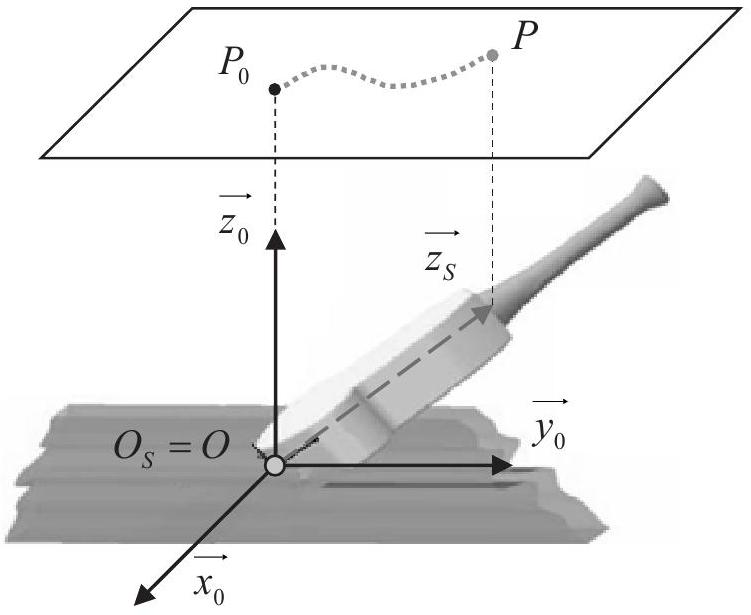
\includegraphics[alt={},max width=\textwidth]{fa0d4e8b-3d38-4fa1-81c7-d2340e1d78c1-17_615_751_313_282}
\captionsetup{labelformat=empty}
\caption{Figure 18 - Trajectoire dans le plan $\left(P_{0}, \overrightarrow{x_{0}}, \overrightarrow{y_{0}}\right)$ du projeté de l'extrémité du vecteur}
\end{center}
\end{figure}

\begin{figure}[h]
\begin{center}
  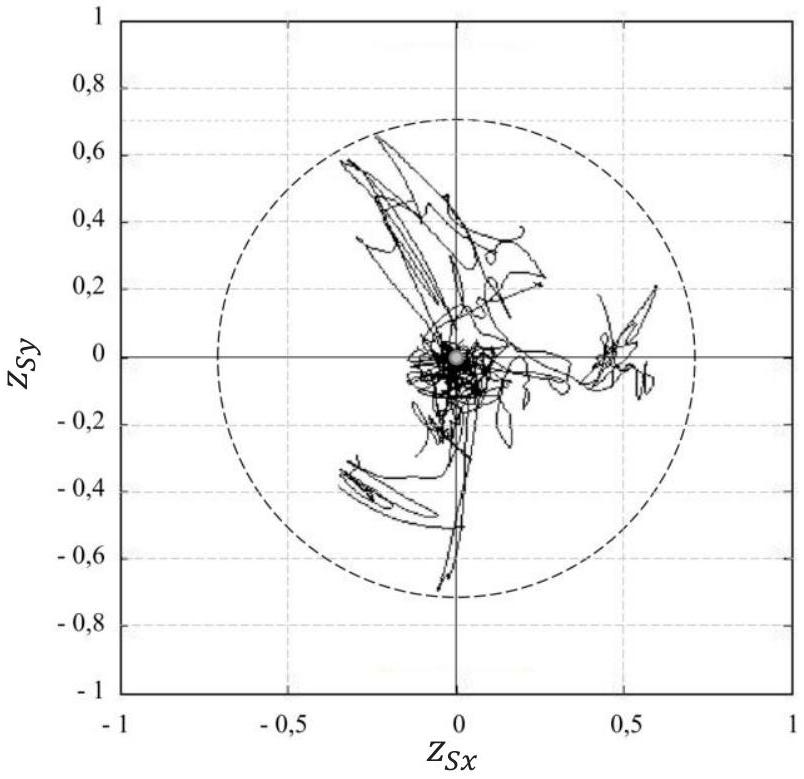
\includegraphics[alt={},max width=\textwidth]{fa0d4e8b-3d38-4fa1-81c7-d2340e1d78c1-17_779_804_216_1061}
\captionsetup{labelformat=empty}
\caption{Figure 19 - Évolution de l'inclinaison de la sonde lors d'un examen d'échographie classique}
\end{center}
\end{figure}

\section*{Distribution statistique des orientations}
La caractérisation de la distribution statistique des orientations au cours de l'examen s'appuie sur l'analyse d'histogrammes ou diagrammes tels que ceux présentés en figure 20. Afin de générer ces tracés, il est nécessaire de procéder à un traitement numérique des mesures. Une phase de prétraitement des résultats permet d'importer les résultats de mesure, de les filtrer, et renvoie :

\begin{itemize}
  \item[-] deux listes de même dimension $N$, theta et dt, contenant respectivement les valeurs $\theta_{i}$ $(i=1 \ldots N)$ d'orientations mesurées, en degrés, comprises dans l'intervalle $I=\left[0, \theta_{\text {max }}\right]$ et les durées $\Delta \mathrm{t}_{\mathrm{i}}$ pendant lesquelles la mesure de l'orientation de la sonde prend la valeur $\theta_{i}$,
  \item[-] la valeur theta\_max de l'angle d'inclinaison maximal $\theta_{\text {max }}$.
\end{itemize}

Pour réaliser l'étude de la distribution des valeurs $\theta_{i}$, l'intervalle $I$ est divisé en $M$ sous-intervalles $I_{j},(j=1 \ldots M)$, d'amplitude $1^{\circ}$ (ou classes), tels que $I_{1}=\left[0,1\left[, I_{j}=\left[j, j+1\left[\right.\right.\right.\right.$ et $I_{M}=\left[M, E\left(\theta_{\text {max }}\right)+1[\right.$, où $E\left(\theta_{\text {max }}\right)$ désigne la partie entière de $\theta_{\text {max }}$.

\begin{itemize}
  \item[Q34.] Écrire une fonction traitement1(theta, dt, theta\_max) qui renvoie une liste classes et une liste temps contenant respectivement les $M$ valeurs $j$ et les durées $d_{j}$ associées à chaque sous-intervalle $I_{j}$.
\end{itemize}

L'exécution du code Python permet alors de générer l'histogramme de la figure 20a. On souhaite compléter l'analyse statistique en déterminant les durées cumulées $d c_{j}$, définies pour un sousintervalle $I_{j}$ par : $\left\{\begin{array}{c}d c_{j}=d c_{j-1}+d_{j}, j=2 \cdots M \\ d c_{1}=d_{1}\end{array}\right.$.

\begin{itemize}
  \item[Q35.] Écrire une fonction traitement2 (temps) qui renvoie une liste cumul\_temps contenant les $M$ valeurs de durées cumulées $d c_{j}$.
  \item[Q36.] Donner alors la suite d'instructions permettant de générer le tracé de la figure 20b, en faisant appel aux deux fonctions traitement1 et traitement2.
\end{itemize}

\begin{itemize}
  \item[Q37.] À partir de la valeur trouvée à la Q33 et de l'analyse des graphes de la figure 20, conclure quant à la pertinence de l'exigence 1.1.2.2.
\end{itemize}

\begin{figure}[h]
\begin{center}
  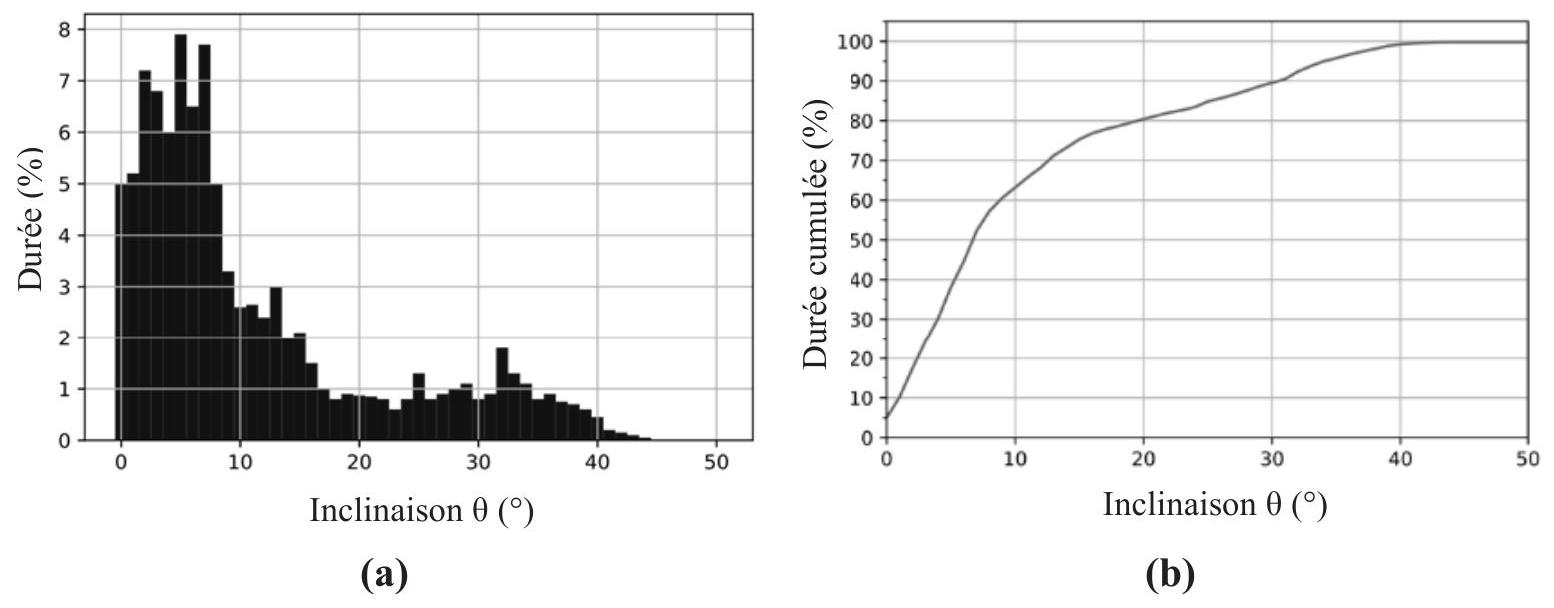
\includegraphics[alt={},max width=\textwidth]{fa0d4e8b-3d38-4fa1-81c7-d2340e1d78c1-18_608_1554_325_248}
\captionsetup{labelformat=empty}
\caption{Figure 20 - Histogramme (a) et diagramme des durées cumulées (b) générés par le code Python}
\end{center}
\end{figure}

\section*{Partie V - Mise en œuvre de la commande distante (Informatique pour tous)}
Les questions d'informatique doivent être traitées en langage Python.

\section*{V. 1 - Génération des lois de mouvement dans l'espace articulaire}
Objectif : générer les lois de commande permettant de satisfaire les exigences 1.2.1.3.1. et 1.2.1.3.2.\\
Loi de commande en vitesse d'un axe\\
On s'intéresse à la génération de mouvement, pour un axe $i$ donné $(i=1 \cdots 3)$, entre deux positions articulaires successives $\theta_{i, k}$ et $\theta_{i, k+1}$. On note $\Delta \theta_{i}=\theta_{i, k+1}-\theta_{i, k}$, l'amplitude angulaire à parcourir, $T_{i}$, le temps nécessaire à l'axe $i$ pour parcourir $\Delta \theta_{i}, v_{i}$ et $a_{i}$, la vitesse et l'accélération maximales de chaque axe $i$. La loi de mouvement est générée à partir d'un profil d'accélération de type " bangbang ", où les phases d'accélération et de freinage sont constantes et symétriques. En fonction des valeurs de $\Delta \theta_{i}, v_{i}$ et $a_{i}$, deux configurations sont possibles : une loi de mouvement sans ou avec palier de vitesse (figure 21).

\begin{itemize}
  \item[Q38.] Pour la loi sans palier de vitesse, déterminer l'expression de la durée $T_{i} / 2$ en fonction de $\Delta \theta_{i}$ et $a_{i}$. Montrer alors qu'une loi sans palier peut être utilisée à la condition que $\Delta \theta i \leq \frac{v_{i}^{2}}{a_{i}}$.
\end{itemize}

Dans le cas où la vitesse maximale $v_{i}$ est atteinte avant l'instant $T_{i} / 2$, on a un palier de vitesse et la durée $T_{i}$ s'exprime : $T_{i}=\frac{\Delta \theta i}{v_{i}}+t_{i}$, avec $t_{i}=\frac{v_{i}}{a_{i}}$.

\begin{itemize}
  \item[Q39.] Écrire une fonction loimvt\_1 (theta\_k, theta\_kp1,v,a) prenant pour arguments d'entrée les positions articulaires successives $\theta_{i, k}$ et $\theta_{i, k+1}$, la vitesse maximale $v_{i}$, l'accélération maximale $a_{i}$ et renvoyant le flottant T associé à la durée $T_{i}$.
\end{itemize}

\section*{Synchronisation des axes du robot}
On souhaite synchroniser les axes 1, 2 et 3 en les réglant sur l'axe le plus lent pour lequel le mouvement a une durée de $T_{\text {max }}$. Cela permet de moins solliciter les actionneurs, sans pour autant augmenter le temps de déplacement de la sonde d'une position à l'autre. Les axes les plus rapides sont ralentis de manière à ce que les mouvements associés se terminent en même temps que celui de l'axe le plus lent. On définit ainsi, pour chaque axe à ralentir, un coefficient de réduction $\eta_{i}$ inférieur à 1 tel que sa nouvelle accélération soit égale à $\eta_{i} a_{i}$.\\
Cela conduit aux expressions suivantes :

\begin{itemize}
  \item[-] pour une loi sans palier : $\eta_{i}=\frac{4 \Delta \theta i}{a_{i} \cdot T_{\text {max }}^{2}}$ et $t_{i}=\frac{T_{\text {max }}}{2}$;
  \item[-] pour une loi avec palier : $\eta_{i}=\frac{v_{i}^{2}}{\left(v_{i} \cdot T_{\text {max }}-\Delta \theta i\right) a_{i}}$ et $t_{i}=\frac{v_{i}}{\eta_{i} a_{i}}$.
\end{itemize}

Q40. Écrire une fonction loimvt\_2(theta\_k, theta\_kp1,v,a,Tmax) prenant pour arguments d'entrée les positions articulaires successives $\theta_{i, k}$ et $\theta_{i, k+1}$, la vitesse maximale $v_{i}$, l'accélération maximale $a_{i}$, la durée $T_{\text {max }}$ et renvoyant les flottants red et ti associés aux valeurs du coefficient de réduction $\eta_{i}$ et de l'instant $t_{i}$ pour l'axe i.

Il est ainsi possible de déterminer les coefficients $\eta_{i}$, les temps $T_{\text {max }}$ et $t_{i}$, pour l'ensemble des 3 axes afin d'élaborer les lois de commande en position à envoyer au contrôleur de chaque axe $i$.

\begin{figure}[h]
\begin{center}
  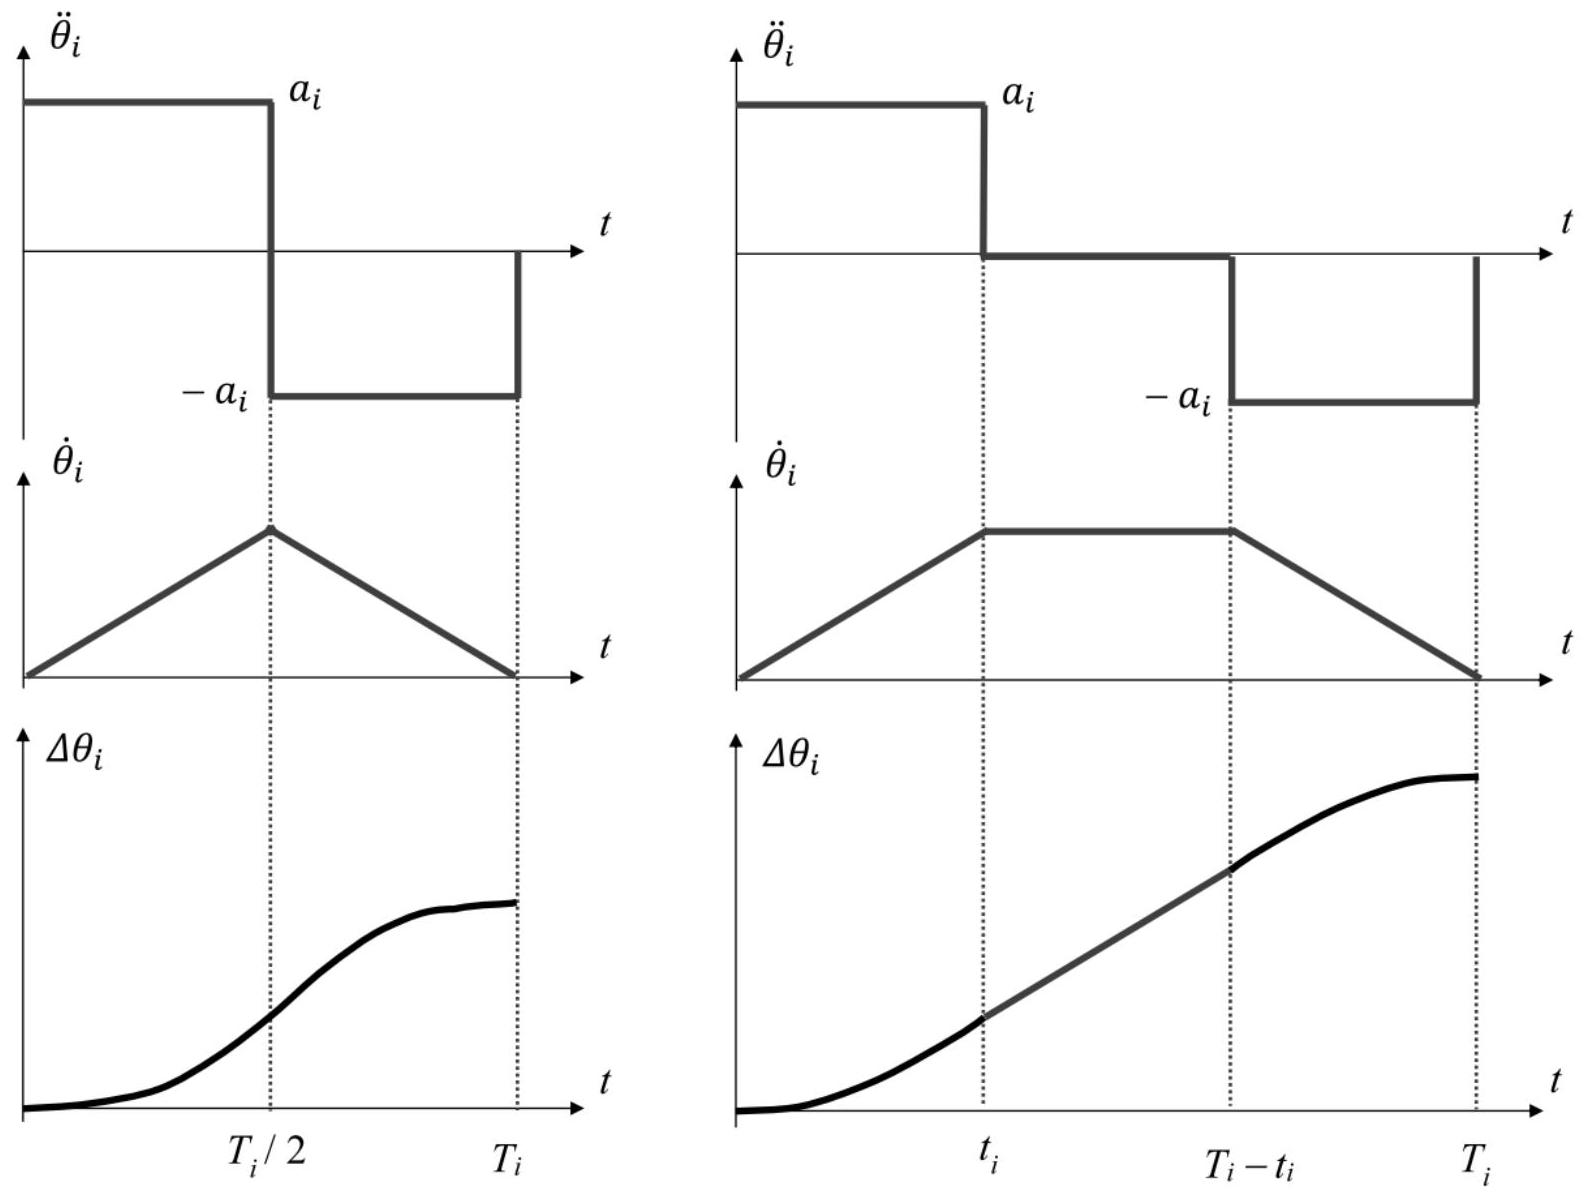
\includegraphics[alt={},max width=\textwidth]{fa0d4e8b-3d38-4fa1-81c7-d2340e1d78c1-19_1196_1587_1445_235}
\captionsetup{labelformat=empty}
\caption{Figure 21 - Loi de mouvement avec ou sans palier de vitesse}
\end{center}
\end{figure}

\section*{V. 2 - Communication entre site expert et site patient}
Objectif : valider les performances de la commande distante (exigence 1.2.3.).\\
La communication entre le site expert et le site patient s'effectue via deux canaux de communication distincts :

\begin{itemize}
  \item[-] un premier canal dédié à la visio-conférence (son et image) et aux images échographiques ;
  \item[-] un second canal pour la commande du robot porte-sonde et l'échange des données de contrôle.
\end{itemize}

On s'intéresse à l'échange des données de contrôle/commande du robot qui met en œuvre un protocole de communication IP.\\
La structure des paquets de données échangés entre les deux postes est décrite sur la figure 22. Les données sont émises au format ASCII. Les paquets sont formatés avec un caractère ASCII d'en-tête, et un caractère de fin.

\begin{figure}[h]
\begin{center}
  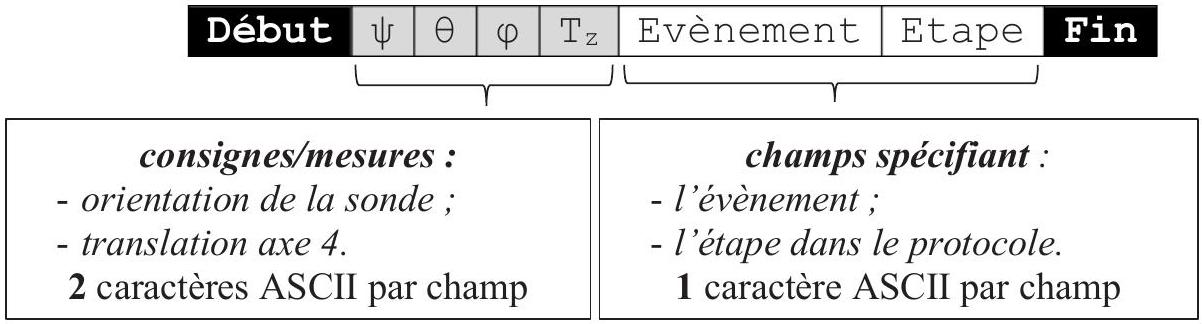
\includegraphics[alt={},max width=\textwidth]{fa0d4e8b-3d38-4fa1-81c7-d2340e1d78c1-20_324_1202_906_411}
\captionsetup{labelformat=empty}
\caption{Figure 22 - Structure des paquets de données échangés}
\end{center}
\end{figure}

\begin{itemize}
  \item[Q41.] Sachant qu'un caractère ASCII est codé sur un octet, déterminer la taille en octets d'un paquet de données.
\end{itemize}

On se place dans la configuration la plus défavorable correspondant à une transmission par satellite, pour laquelle on dispose d'un débit de données limité à $64 \mathrm{~kb} / \mathrm{s}(1 \mathrm{~kb} / \mathrm{s}=1000 \mathrm{bit} / \mathrm{s})$.

\begin{itemize}
  \item[Q42.] Calculer la fréquence $f$ à laquelle il est possible de travailler avec ce mode de transmission. Commenter la valeur trouvée, sachant qu'au-delà de 320 Hz le doigt humain n'est plus en mesure de discriminer deux signaux de force consécutifs.
\end{itemize}

\section*{Synthèse globale de l'étude}
\begin{itemize}
  \item[Q43.] En prenant comme point de départ l'objectif global fixé et la démarche proposée présentés en page 4, réaliser une synthèse reprenant les différents points abordés dans le cadre de cette étude. Conclure sur l'aptitude des solutions retenues à satisfaire les exigences du cahier des charges abordées au cours de l'étude.
\end{itemize}

\section*{FIN}
\begin{center}
\begin{tabular}[t]{|L{0.45\textwidth}|L{0.45\textwidth}|}
\hline
\begin{tabular}[t]{L{0.9\linewidth}}
Numéro
\includegraphics[max width=\textwidth, alt={}]{fa0d4e8b-3d38-4fa1-81c7-d2340e1d78c1-21_203_227_118_102}
 \\
d'inscription\begin{tabular}[t]{|L{0.18\linewidth}|L{0.18\linewidth}|L{0.18\linewidth}|L{0.18\linewidth}|L{0.18\linewidth}|}
\hline
 &  &  &  &  \\
\hline
\end{tabular} Nom : \_\_\_\_ \\
Numéro de table\begin{tabular}[t]{|L{0.15\linewidth}|L{0.15\linewidth}|L{0.15\linewidth}|L{0.15\linewidth}|L{0.15\linewidth}|L{0.15\linewidth}|}
\hline
 &  &  &  &  &  \\
\hline
\end{tabular} Prénom : \_\_\_\_ \\
Né(e) le\begin{tabular}[t]{|L{0.45\linewidth}|L{0.45\linewidth}|}
\hline
 &  \\
\hline
\end{tabular}\begin{tabular}[t]{|L{0.45\linewidth}|L{0.45\linewidth}|}
\hline
 &  \\
\hline
\end{tabular}\begin{tabular}[t]{|L{0.23\linewidth}|L{0.23\linewidth}|L{0.23\linewidth}|L{0.23\linewidth}|}
\hline
 &  &  &  \\
\hline
\end{tabular} \\
Emplacement OR Code \\
\end{tabular} & \begin{tabular}[t]{L{0.9\linewidth}}
\begin{tabular}[t]{|L{0.45\linewidth}|L{0.45\linewidth}|}
\hline
Filière : & MP \\
\hline
\end{tabular} \\
Session : 2021 \\
Épreuve de : Sciences Industrielles

\begin{itemize}[leftmargin=*, topsep=0pt, itemsep=0pt, parsep=0pt, partopsep=0pt]
  \item[-] Remplir soigneusement l'en-tête de chaque feuille avant de commencer à composer
  \item[-] Rédiger avec un stylo non effaçable bleu ou noir
  \item[-] Ne rien écrire dans les marges (gauche et droite)
  \item[-] Numéroter chaque page (cadre en bas à droite)
  \item[-] Placer les feuilles A3 ouvertes, dans le même sens et dans l'ordre
\end{itemize} \\
\end{tabular} \\
\hline
\end{tabular}
\end{center}

\section*{DOCUMENT RÉPONSE}
Ce Document Réponse doit être rendu dans son intégralité avec la copie.

DR 1 - Schéma bloc de l'asservissement en vitesse de l'axe 1\\
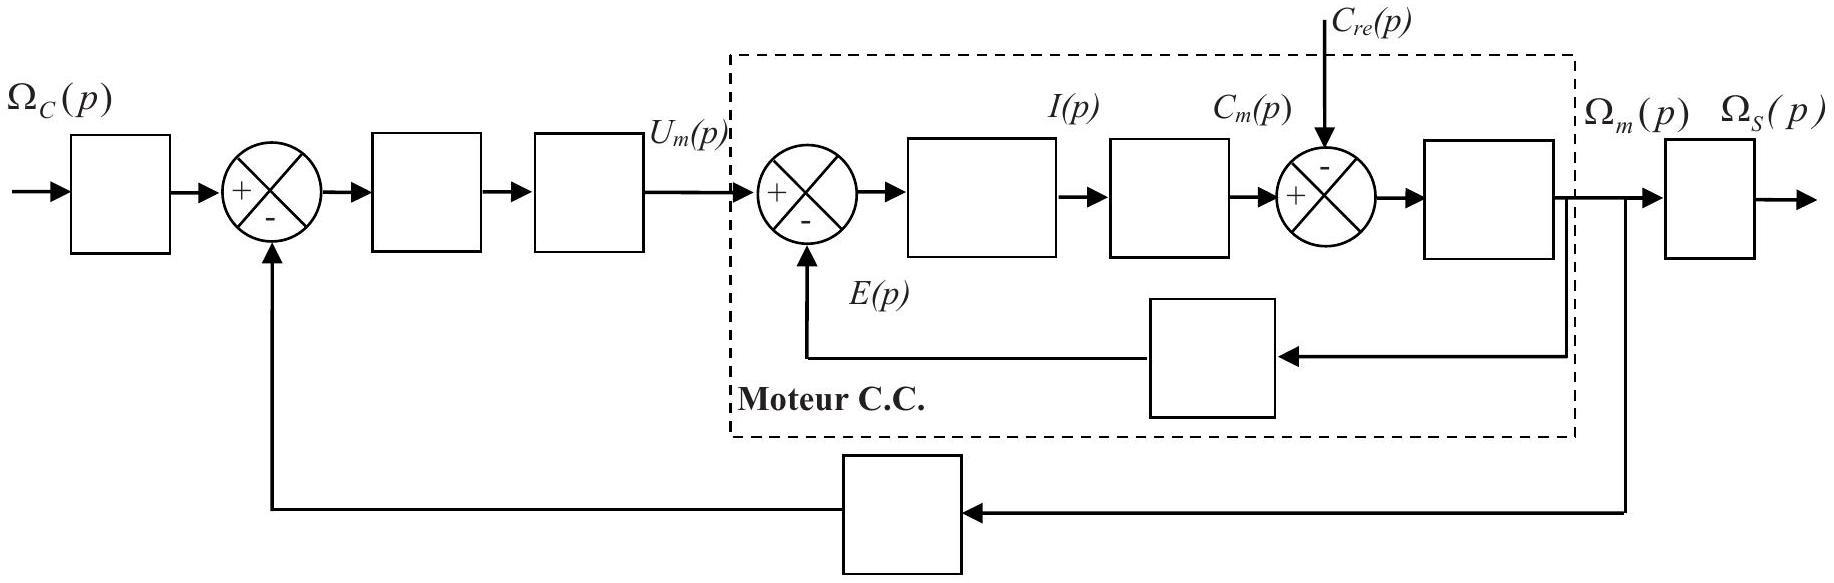
\includegraphics[max width=\textwidth, alt={}, center]{fa0d4e8b-3d38-4fa1-81c7-d2340e1d78c1-21_583_1834_1940_143}

\section*{NE RIEN ÉCRIRE DANS CE CADRE}
\begin{figure}[h]
\begin{center}
\captionsetup{labelformat=empty}
\caption{DR 2 - Diagramme de Bode}
  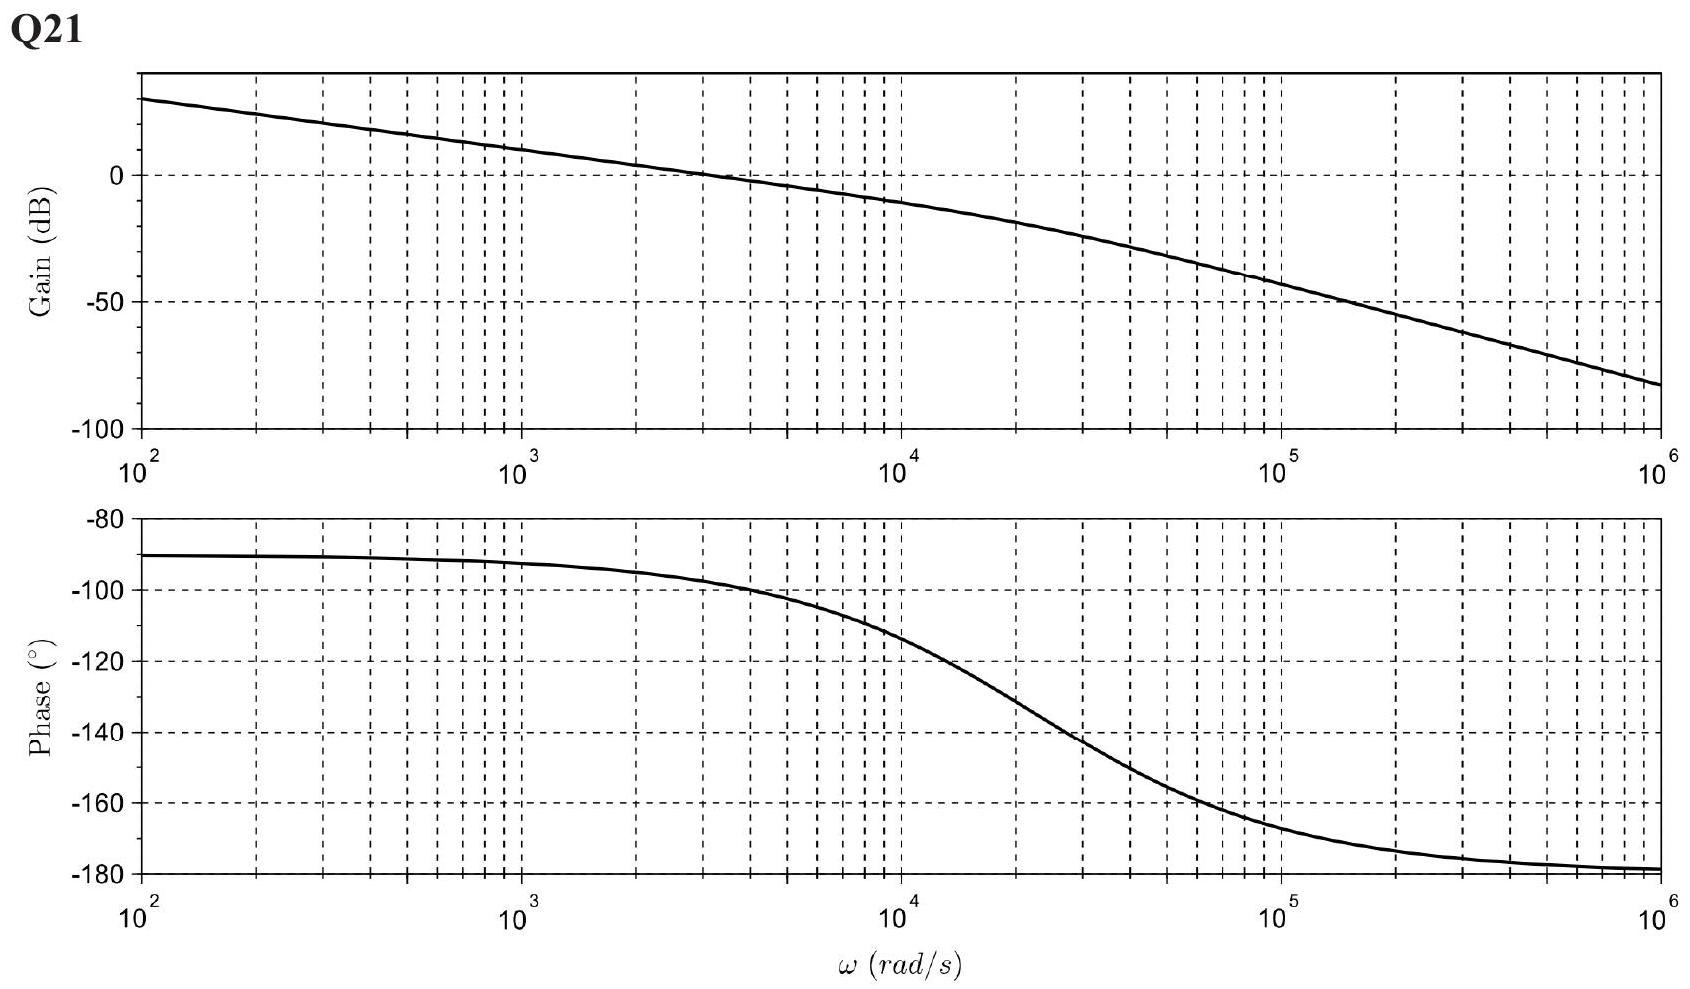
\includegraphics[alt={},max width=\textwidth]{fa0d4e8b-3d38-4fa1-81c7-d2340e1d78c1-22_989_1690_535_186}
\end{center}
\end{figure}

Marge de gain : Marge de phase :

\begin{figure}[h]
\begin{center}
\captionsetup{labelformat=empty}
\caption{DR 3 - Réponses temporelles : boucle de vitesse}
  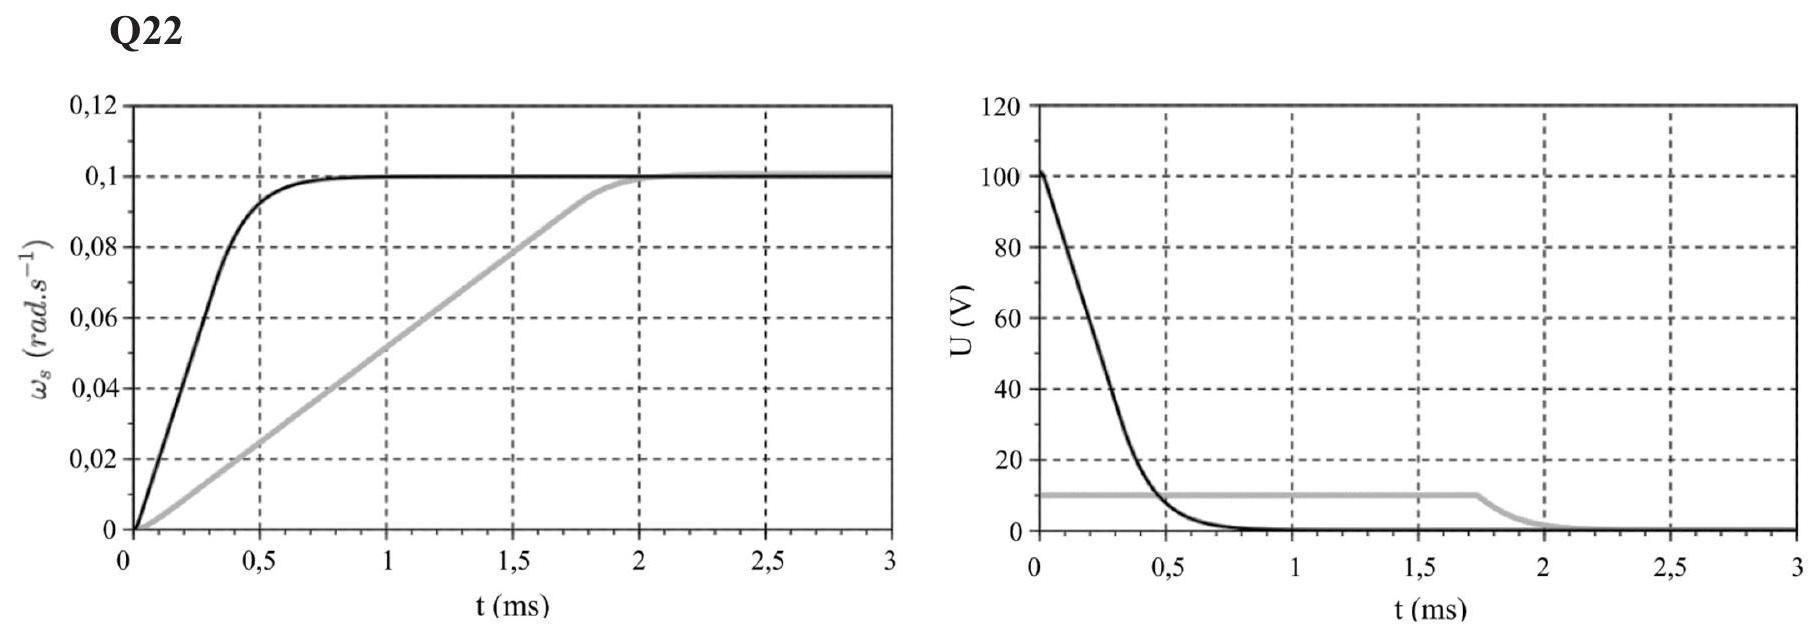
\includegraphics[alt={},max width=\textwidth]{fa0d4e8b-3d38-4fa1-81c7-d2340e1d78c1-22_633_1818_1944_87}
\end{center}
\end{figure}

Q24

\begin{figure}[h]
\begin{center}
\captionsetup{labelformat=empty}
\caption{DR 4 - Réponse temporelle : boucle de position}
  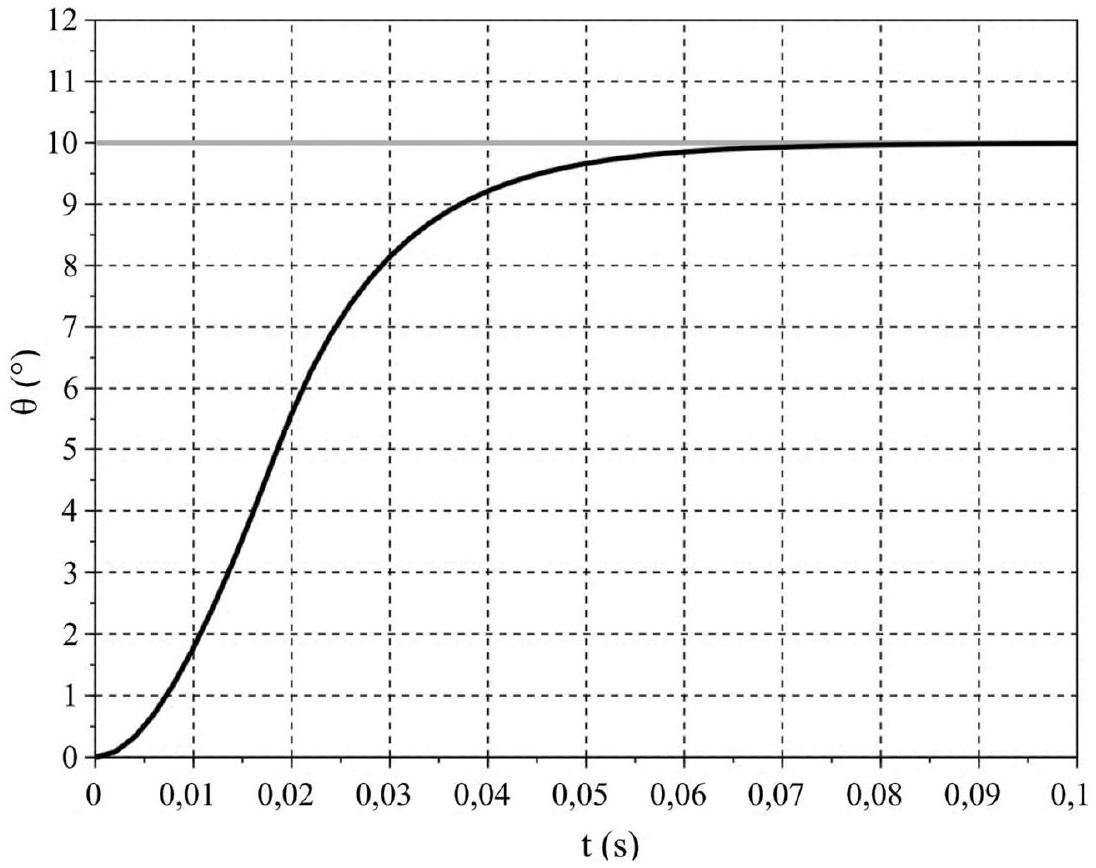
\includegraphics[alt={},max width=\textwidth]{fa0d4e8b-3d38-4fa1-81c7-d2340e1d78c1-23_868_1096_434_484}
\end{center}
\end{figure}

\begin{figure}[h]
\begin{center}
\captionsetup{labelformat=empty}
\caption{req [Modèle] ROBOT TELE-ECHOGRAPHIE[ Diagramme d'exigences}
  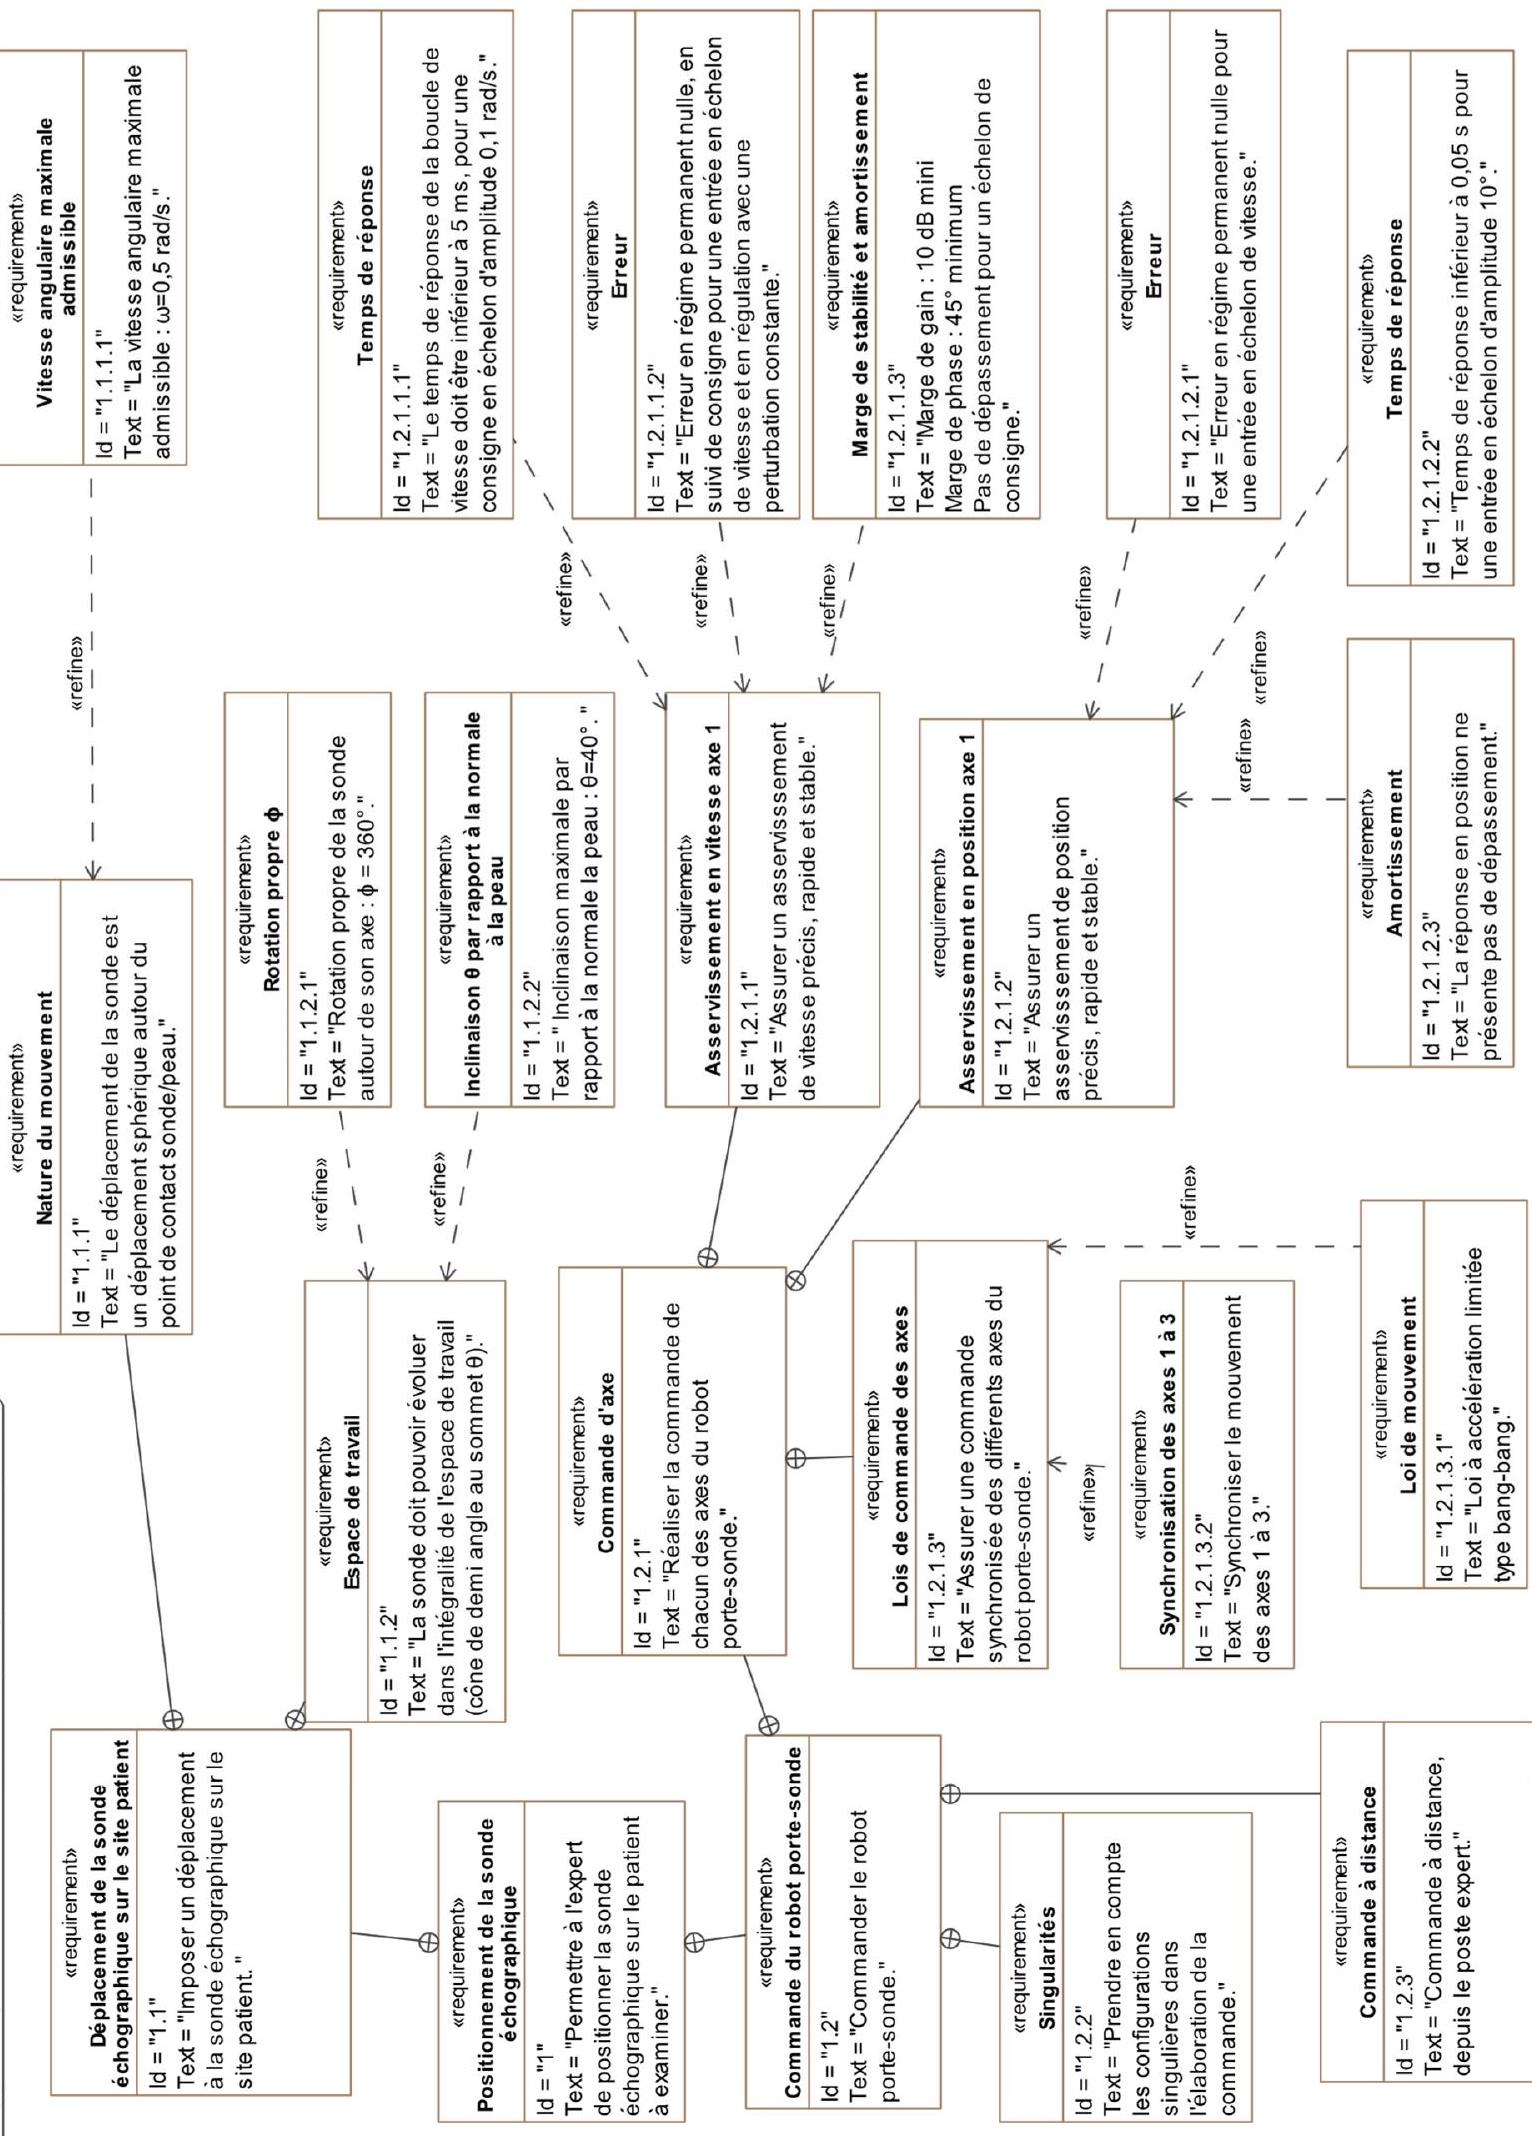
\includegraphics[alt={},max width=\textwidth]{fa0d4e8b-3d38-4fa1-81c7-d2340e1d78c1-24_2136_1532_483_249}
\end{center}
\end{figure}


\end{document}